% SIAM Supplemental File Template
\documentclass[review,supplement,onefignum,onetabnum]{siamonline220329}

% SIAM Shared Information Template
% This is information that is shared between the main document and any
% supplement. If no supplement is required, then this information can
% be included directly in the main document.


% Packages and macros go here
\usepackage[utf8]{inputenc} % allow utf-8 input
\usepackage[T1]{fontenc}    % use 8-bit T1 fonts
% \usepackage{hyperref}       % hyperlinks
\usepackage{url}            % simple URL typesetting
\usepackage{booktabs}       % professional-quality tables
\usepackage{amsfonts}       % blackboard math symbols
\usepackage{nicefrac}       % compact symbols for 1/2, etc.
\usepackage{microtype}      % microtypography
\usepackage{lipsum}
\usepackage{graphicx}
\let\subcaption\relax
\usepackage{caption}
\usepackage{subcaption}
% \usepackage{subfigure}
\usepackage{amsmath}
\usepackage{amssymb}
\usepackage{mathtools}




\usepackage{hyperref}
\usepackage{xr}
% \usepackage{subfig}
\usepackage{xcolor}
\usepackage{multirow}
% \usepackage{ulem}

\DeclareMathOperator*{\argmax}{arg\,max}
\DeclareMathOperator*{\argmin}{arg\,min}
\DeclareMathOperator{\score}{score}

% Algorithmic modifications for loop and break


% Note that the amsmath package sets \interdisplaylinepenalty to 10000
% thus preventing page breaks from occurring within multiline equations. Use:
\interdisplaylinepenalty=2500
% after loading amsmath to restore such page breaks as IEEEtran.cls normally
% does. amsmath.sty is already installed on most LaTeX systems. The latest
% version and documentation can be obtained at:
% http://www.ctan.org/pkg/amsmath

\usepackage{placeins}
\usepackage{xr}
\usepackage{hyperref}
\usepackage{lipsum}
\usepackage{amsfonts}
\usepackage{graphicx}
\usepackage{epstopdf}
\usepackage{algpseudocode}
\ifpdf
  \DeclareGraphicsExtensions{.eps,.pdf,.png,.jpg}
\else
  \DeclareGraphicsExtensions{.eps}
\fi

% Prevent itemized lists from running into the left margin inside theorems and proofs
\usepackage{enumitem}
\setlist[enumerate]{leftmargin=.5in}
\setlist[itemize]{leftmargin=.5in}

% Add a serial/Oxford comma by default.
\newcommand{\creflastconjunction}{, and~}

% Used for creating new theorem and remark environments
\newsiamremark{remark}{Remark}
\newsiamremark{hypothesis}{Hypothesis}
\crefname{hypothesis}{Hypothesis}{Hypotheses}
\newsiamthm{claim}{Claim}

% Sets running headers as well as PDF title and authors
\headers{CAKES: Scalable, Exact Search on Big Data}{M. E. Prior, T. J. Howard III, O. McLaughlin, T. Ferguson, N. Ishaq, N. M. Daniels}

% Title. If the supplement option is on, then "Supplementary Material"
% is automatically inserted before the title.
\title{Let them have CAKES: A Cutting-Edge Algorithm for Scalable, Efficient, and Exact Search on Big Data\thanks{Submitted to the editors DATE.
}}

\author{
    Morgan E. Prior\thanks{
    Department of Mathematics,
    University of Rhode Island,
    Kingston, RI
    (\email{meprior424@gmail.com})}
    \and
    Thomas J. Howard III\thanks{
    Department of Computer Science and Statistics,
    University of Rhode Island,
    Kingston, RI
    (\email{thoward27@uri.edu}, \email{olwmc@gmail.com}, \email{fergusontr@gmail.com}, \email{najib\_ishaq@zoho.com}, \email{noah\_daniels@uri.edu})}
    \and
    Oliver McLaughlin\footnotemark[3]
    \and
    Terrence Ferguson\footnotemark[3]
    \and
    Najib Ishaq\footnotemark[3]
    \and
    Noah M. Daniels\footnotemark[3]
}


\usepackage{amsopn}
\DeclareMathOperator{\diag}{diag}


%%% Local Variables: 
%%% mode:latex
%%% TeX-master: "ex_article"
%%% End: 

\begin{document}
% Optional PDF information
\ifpdf
\hypersetup{
  pdftitle={Supplementary Materials: Let them have CAKES: A Cutting-Edge Algorithm for Scalable, Efficient, and Exact Search on Big DataAn Example Article},
  pdfauthor={M. E. Prior, T. J. Howard III, O. McLaughlin, T. Ferguson, N. Ishaq, N. M. Daniels}
}
\fi


\maketitle


\section{Supplementary Methods}

% \subsection{\texorpdfstring{$\rho$}{p}-Nearest Neighbors Search}

% We conduct $\rho$-NN search as described in~\cite{ishaq2019clustered}, but with the following improvement:
% when a cluster overlaps with the query ball, instead of always proceeding to search both of its children, we proceed only with those children that might contain points in the query ball.

% \begin{figure}[ht!]
%     \centering
%     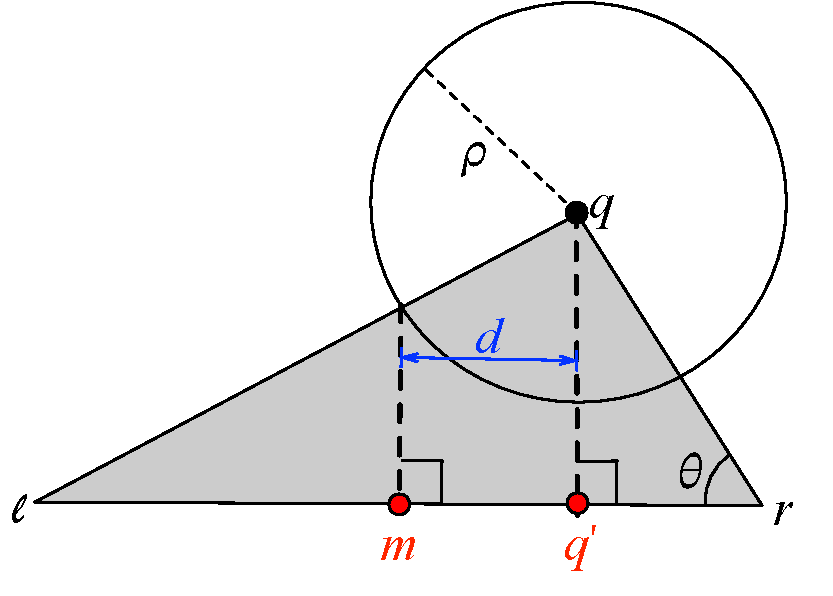
\includegraphics[scale=0.75]{images/geometry/overlapping-children-3.pdf}
%     \caption{The geometry of a query ball overlapping with a cluster and either one or both of its children. Here, $l$ is the left pole, $r$ is the right pole, and $q$ is the query. Other points and distances are described in the text.}
%     \label{fig:methods:overlapping-children}
%     \caption{CAKES uses geometric properties of clusters.}
% \end{figure}

% To determine whether both children can contain points in the query ball, we consider Figure~\ref{fig:methods:overlapping-children}.
% Here, we overload the notation for $\overline{x y}$ to refer both to the line segment joining points $x$ and $y$ as well as to the length of that line segment.

% Let $q$ denote the query, $\rho$ denote the search radius, and $l$ and $r$ denote the cluster's left and right poles respectively (see Section~\ref{sec:methods:clustering:building-the-tree}).
% Without loss of generality, we assume that $\overline{q r \vphantom{l}} \leq \overline{q l}$.
% Now let $q'$ be the projection of $q$ onto $\overline{l r}$, $m$ be the midpoint of $\overline{l r}$, and $d$ be the distance from $q'$ to $m$.
% As a consequence of how we assign a point in the parent cluster to the left child in Algorithm~\ref{alg:methods:partition}, if $\rho < d$, then the left child cannot contain points inside the query ball.
% In such a case we proceed to search only the right child.
% Otherwise, we proceed with both children.

% To check whether $d \leq \rho$, we note that $d = \overline{m q' \vphantom{l}} = \overline{m r \vphantom{l}} - \overline{q' r \vphantom{l}} = \frac{\overline{l r}}{2} - \overline{q' r \vphantom{l}}$.
% Let $\theta$ denote $\angle l r q$, as shown in Figure~\ref{fig:methods:overlapping-children}.
% By the Law of Cosines on $\triangle l r q$, we have that $\text{cos}(\theta) = \tfrac{\overline{l r}^2 + \ \overline{q r \vphantom{l}}^2 - \ \overline{q l}^2}{2 \cdot \overline{l r} \cdot \overline{q r \vphantom{l}}}$.
% Since $\triangle r q q'$ is a right triangle, we also have that $\text{cos}(\theta) = \tfrac{\overline{q' r \vphantom{l}}}{\overline{q r \vphantom{l}}}$.
% Combining the previous two equations and solving for $\overline{q' r \vphantom{l}}$, we have that $\overline{q' r \vphantom{l}} = \tfrac{\overline{q r \vphantom{l}}^2 + \ \overline{l r}^2 - \ \overline{q l}^2}{2 \cdot \overline{l r}}$.
% Substituting for $\overline{q' r \vphantom{l}}$ in the equation for $d$, we have that $d = \tfrac{\overline{l r}}{2} - \tfrac{\overline{q r \vphantom{l}}^2 + \ \overline{l r}^2 - \ \overline{q l}^2}{2 \cdot \overline{l r}} = \tfrac{\overline{q l}^2 - \overline{q r \vphantom{l}}^2}{2 \cdot \overline{l r}}$.


% Thus, $d \leq \rho \iff (\overline{q l} + \overline{q r \vphantom{l}})(\overline{q l} - \overline{q r \vphantom{l}}) \leq 2 \cdot \overline{l r} \cdot \rho$. Note, in particular, that this only requires distances between actual points from the dataset, and so it can be used with any distance function, even when $q'$ and $m$ are not actual points or cannot be imputed from the data.

% To perform $\rho$-NN search, we first perform a coarse \textit{tree-search}, as outlined in Algorithm~\ref{alg:methods:rnn-search:tree-search}, to find the leaf clusters that overlap with the query ball or any clusters which lie entirely within the query ball.
% Then, for all such clusters, we perform a finer-grained \textit{leaf-search}, as outlined in Algorithm~\ref{alg:methods:rnn-search:leaf-search}, to find all points that are no more than a distance $\rho$ from the query.
% The asymptotic complexity of $\rho$-NN is the same as in~\cite{ishaq2019clustered} and shown in Equation~\ref{eq:methods:rnn-search-complexity}.

% \begin{gather}
%     \mathcal{O}
%     \Bigg(
%         \underbrace{
%             \log~\overbrace{\mathcal{N}_{\hat{r}}(X)}^{\textrm{metric entropy}}
%         }_{\textrm{tree-search}}
%         \ + \
%         \underbrace{
%             \overbrace{ \big| B_X(q, \rho) \big|}^{\textrm{output size}}
%             \overbrace{ \left( \frac{\rho + 2 \cdot \hat{r}}{ \rho} \right) ^ d}^{\textrm{scaling factor}}
%         }_{\textrm{leaf-search}}
%     \Bigg)
%     \label{eq:methods:rnn-search-complexity}
% \end{gather}
% where $\hat{r}$ is the \textit{mean} radius of leaf clusters, $\mathcal{N}_{\hat{r}}(X)$ is the metric entropy at that radius, $B_X(q, \rho)$ is a ball of radius $\rho$ around the query $q$, and $d$ is the LFD around the query at the length scale of $\rho$ and $\rho + 2 \cdot \hat{r}$.


\section{Supplementary Results}

\subsection{Indexing and Tuning}

The plots in Figure~\ref{fig:supplement:indexing} show the results of these benchmarks.
The horizontal axis in each subplot shows the cardinality of the dataset augmented with synthetic points.
The left-most point on each line is at the cardinality of the original dataset without any synthetic augmentation.
The vertical axis denotes the sum of indexing and tuning time in seconds.
Both axes are on a logarithmic scale.
Hereafter, when we refer to the ``indexing time'' of an algorithm, we are implicitly referring to the sum of indexing and tuning time for said algorithm.

On all datasets, we observe that the indexing time for CAKES increases roughly linearly as cardinality increases.
HNSW and ANNOY have the slowest indexing times across all the algorithms we benchmarked for each of the four datasets, at each cardinality.
On some datasets, HNSW and ANNOY exhibit indexing times which are orders of magnitude slower than that of CAKES.
FAISS-Flat exhibits the fastest indexing time on each dataset.
This is not surprising, however, given that FAISS-Flat is a na\"{\i}ve linear search algorithm and is not building an index.

We also highlight some differences in indexing time between different datasets.
With Fashion-Mnist, as shown in Figure~\ref{fig:supplement:fashion-mnist-indexing}, we observe that the indexing time for CAKES is faster than that of FAISS-IVF for all cardinalities.
With Glove-25 (see Figure~\ref{fig:supplement:glove-25-indexing}), however, at cardinalities greater than $10^7$, FAISS-IVF has faster indexing time than CAKES.
With Sift, CAKES's indexing time is faster than that of FAISS-IVF until a cardinality of nearly $10^8$, and with the Random dataset, we observe that CAKES has faster indexing time than FAISS-IVF until a cardinality of nearly $10^7$.

\begin{figure}
    \begin{subfigure}[b]{0.47\textwidth}
        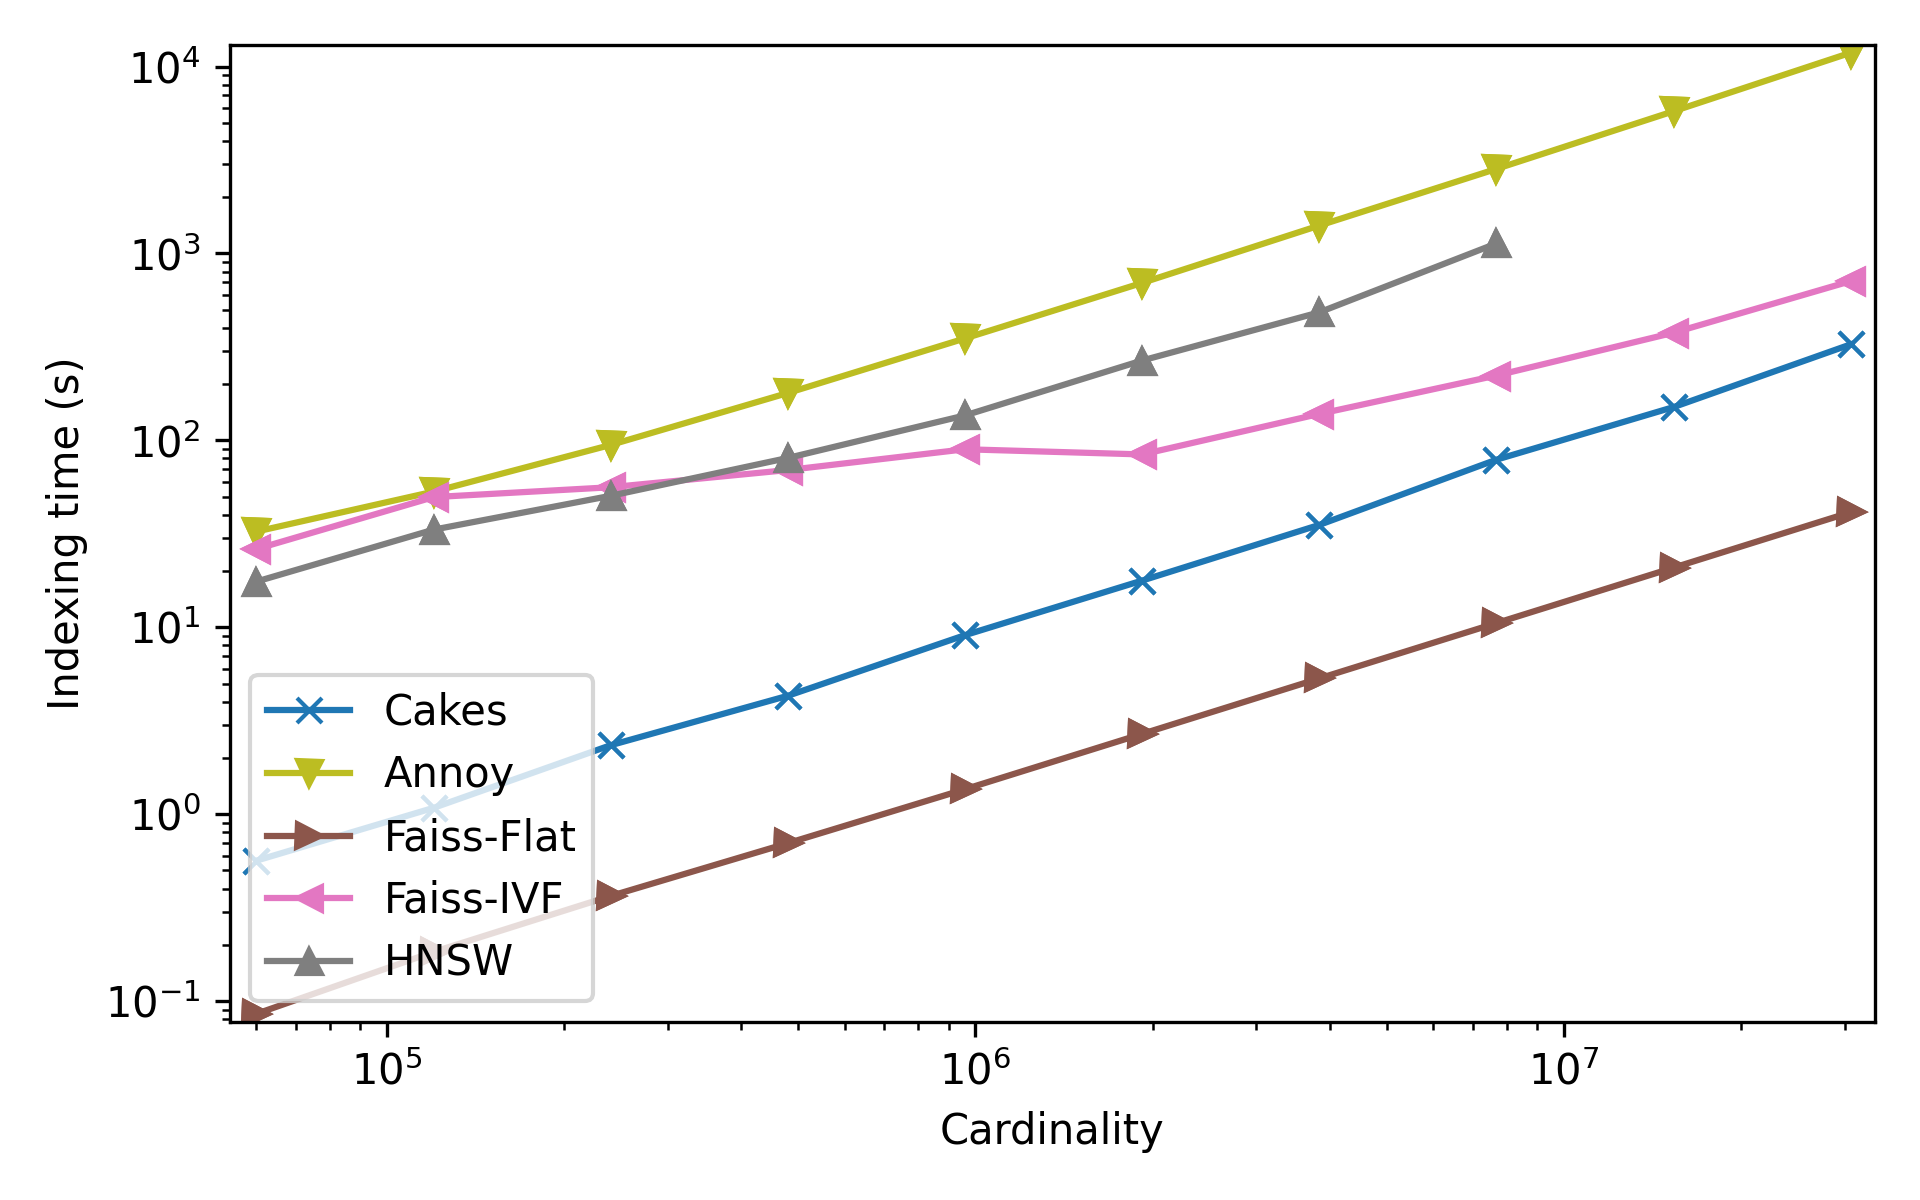
\includegraphics[width=0.95\textwidth]{plots/fashion-mnist-indexing.png}\\
        \subcaption{Fashion-mnist}
        \label{fig:supplement:fashion-mnist-indexing}
    \end{subfigure}%
    \begin{subfigure}[b]{0.47\textwidth}
        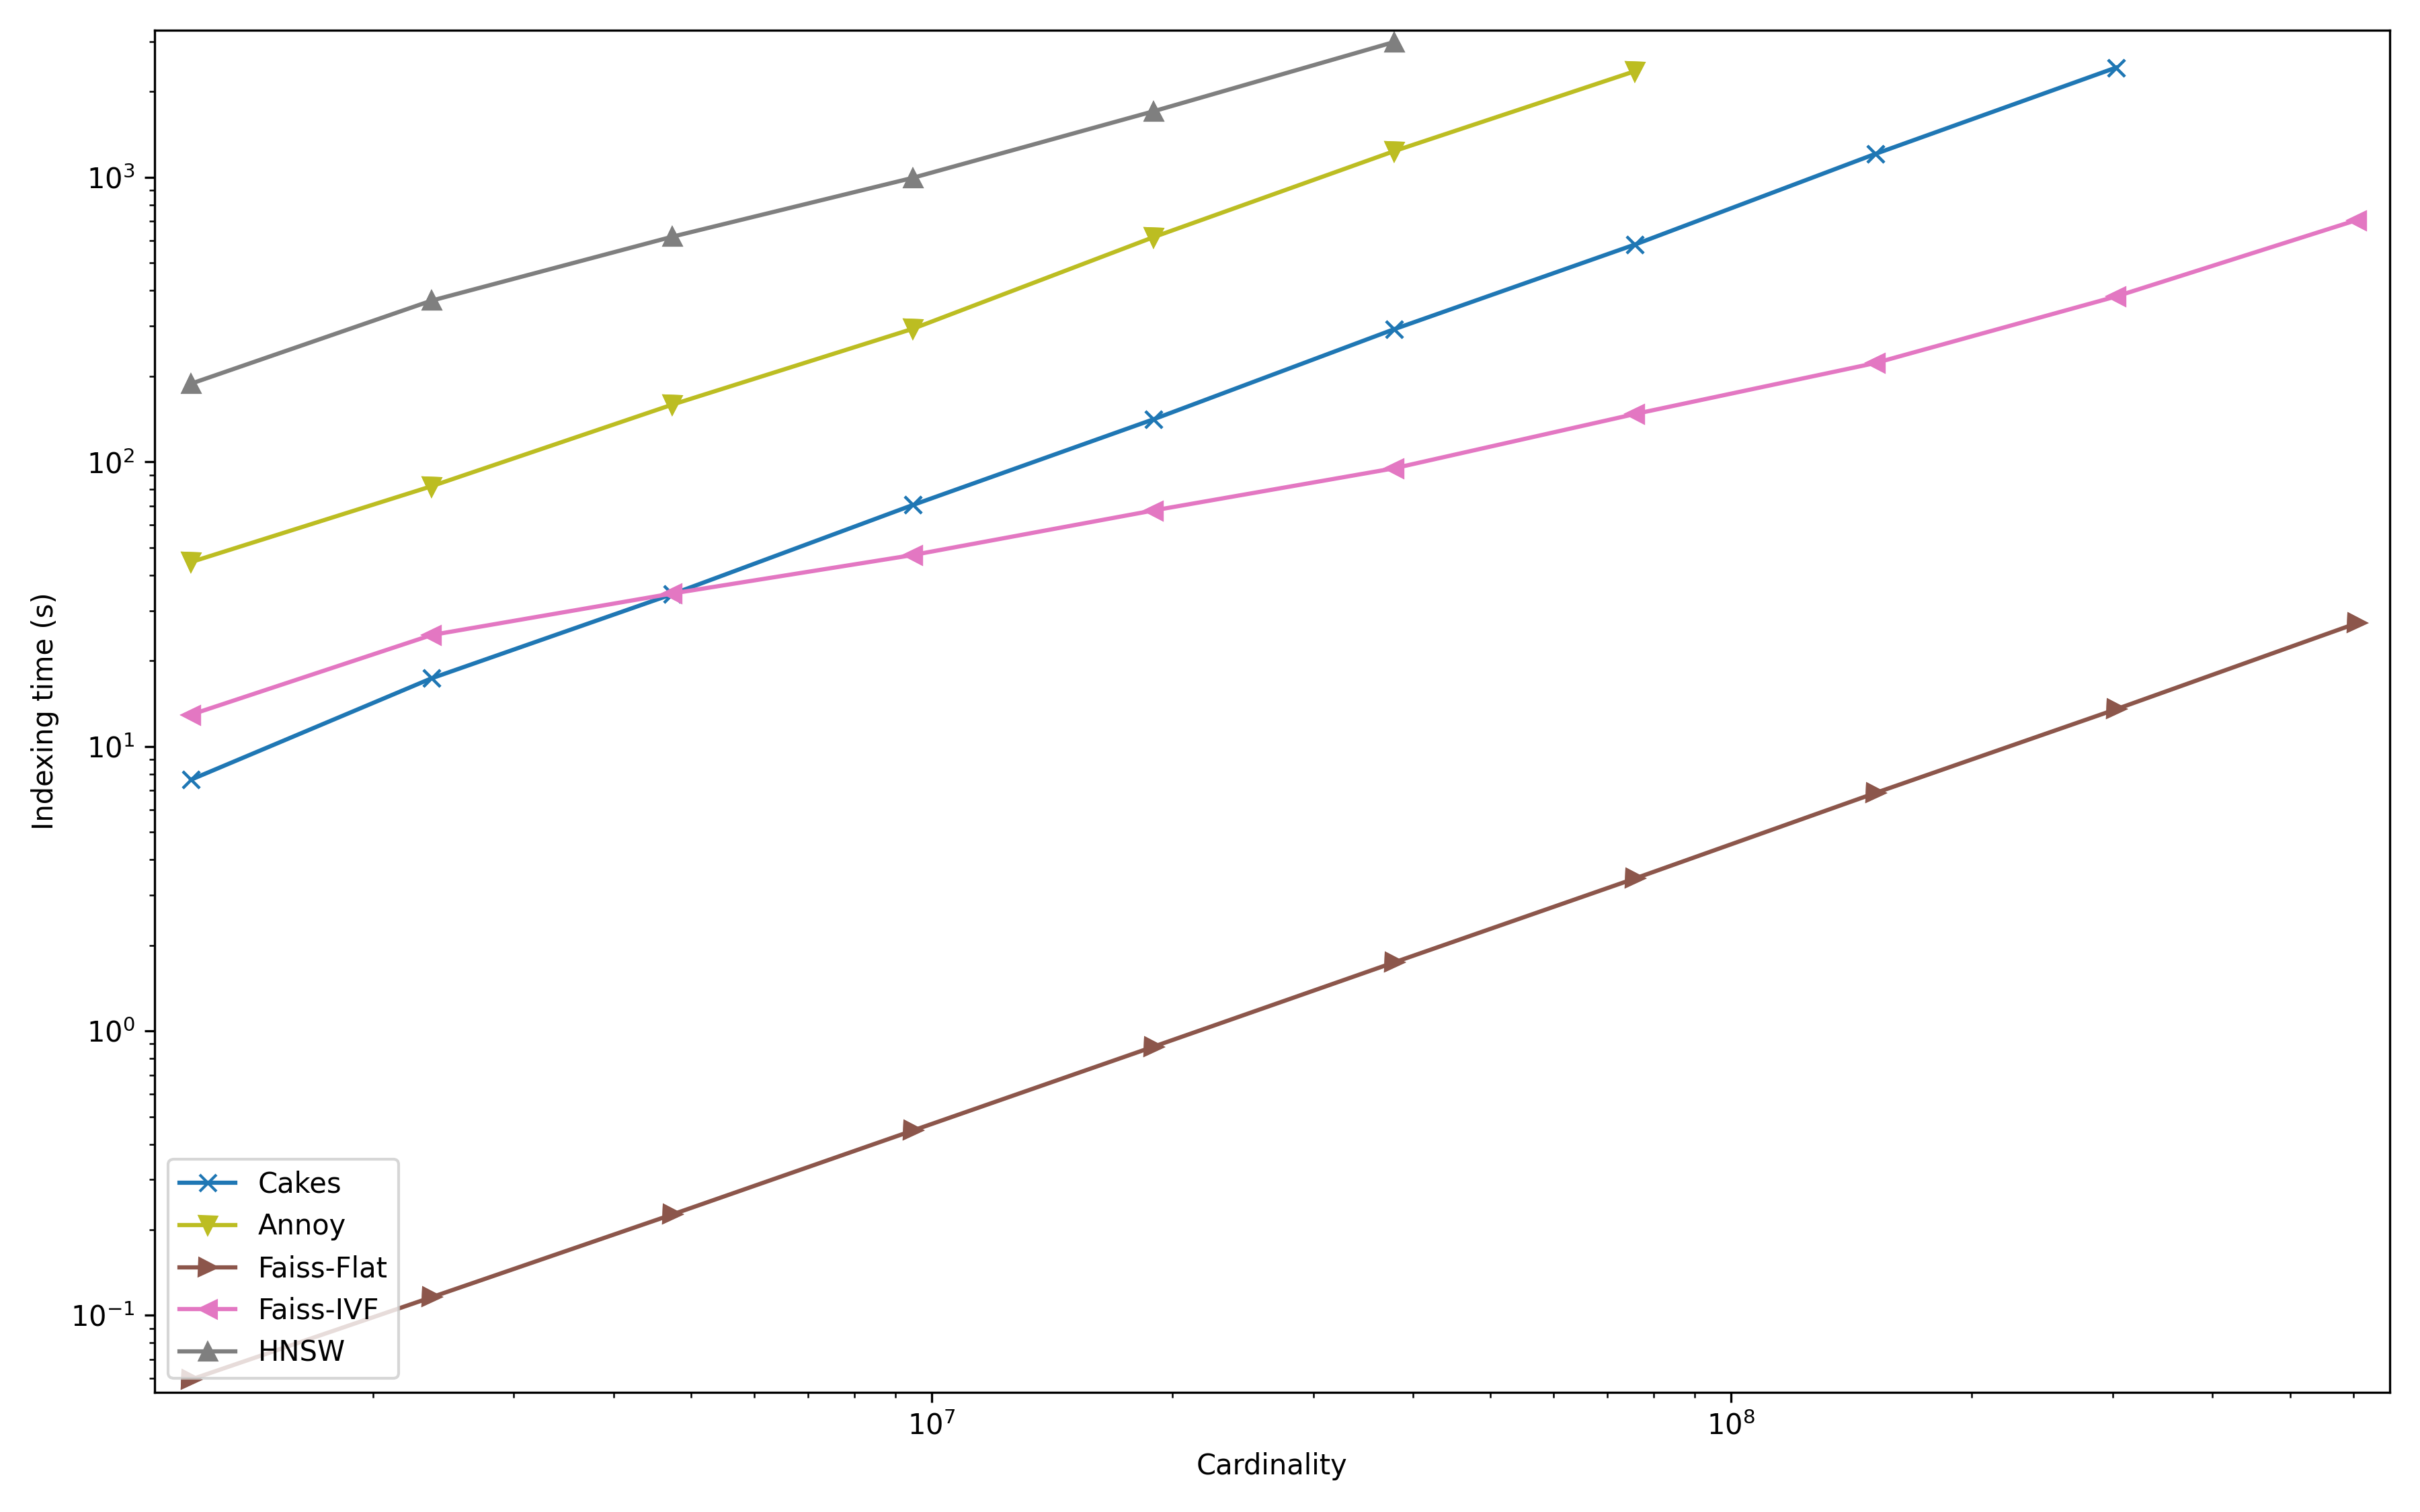
\includegraphics[width=0.95\textwidth]{plots/glove-25-indexing.png}\\
        \subcaption{Glove-25}
        \label{fig:supplement:glove-25-indexing}
    \end{subfigure}
    \vspace{1em}
    \\
    \begin{subfigure}[b]{0.47\textwidth}
        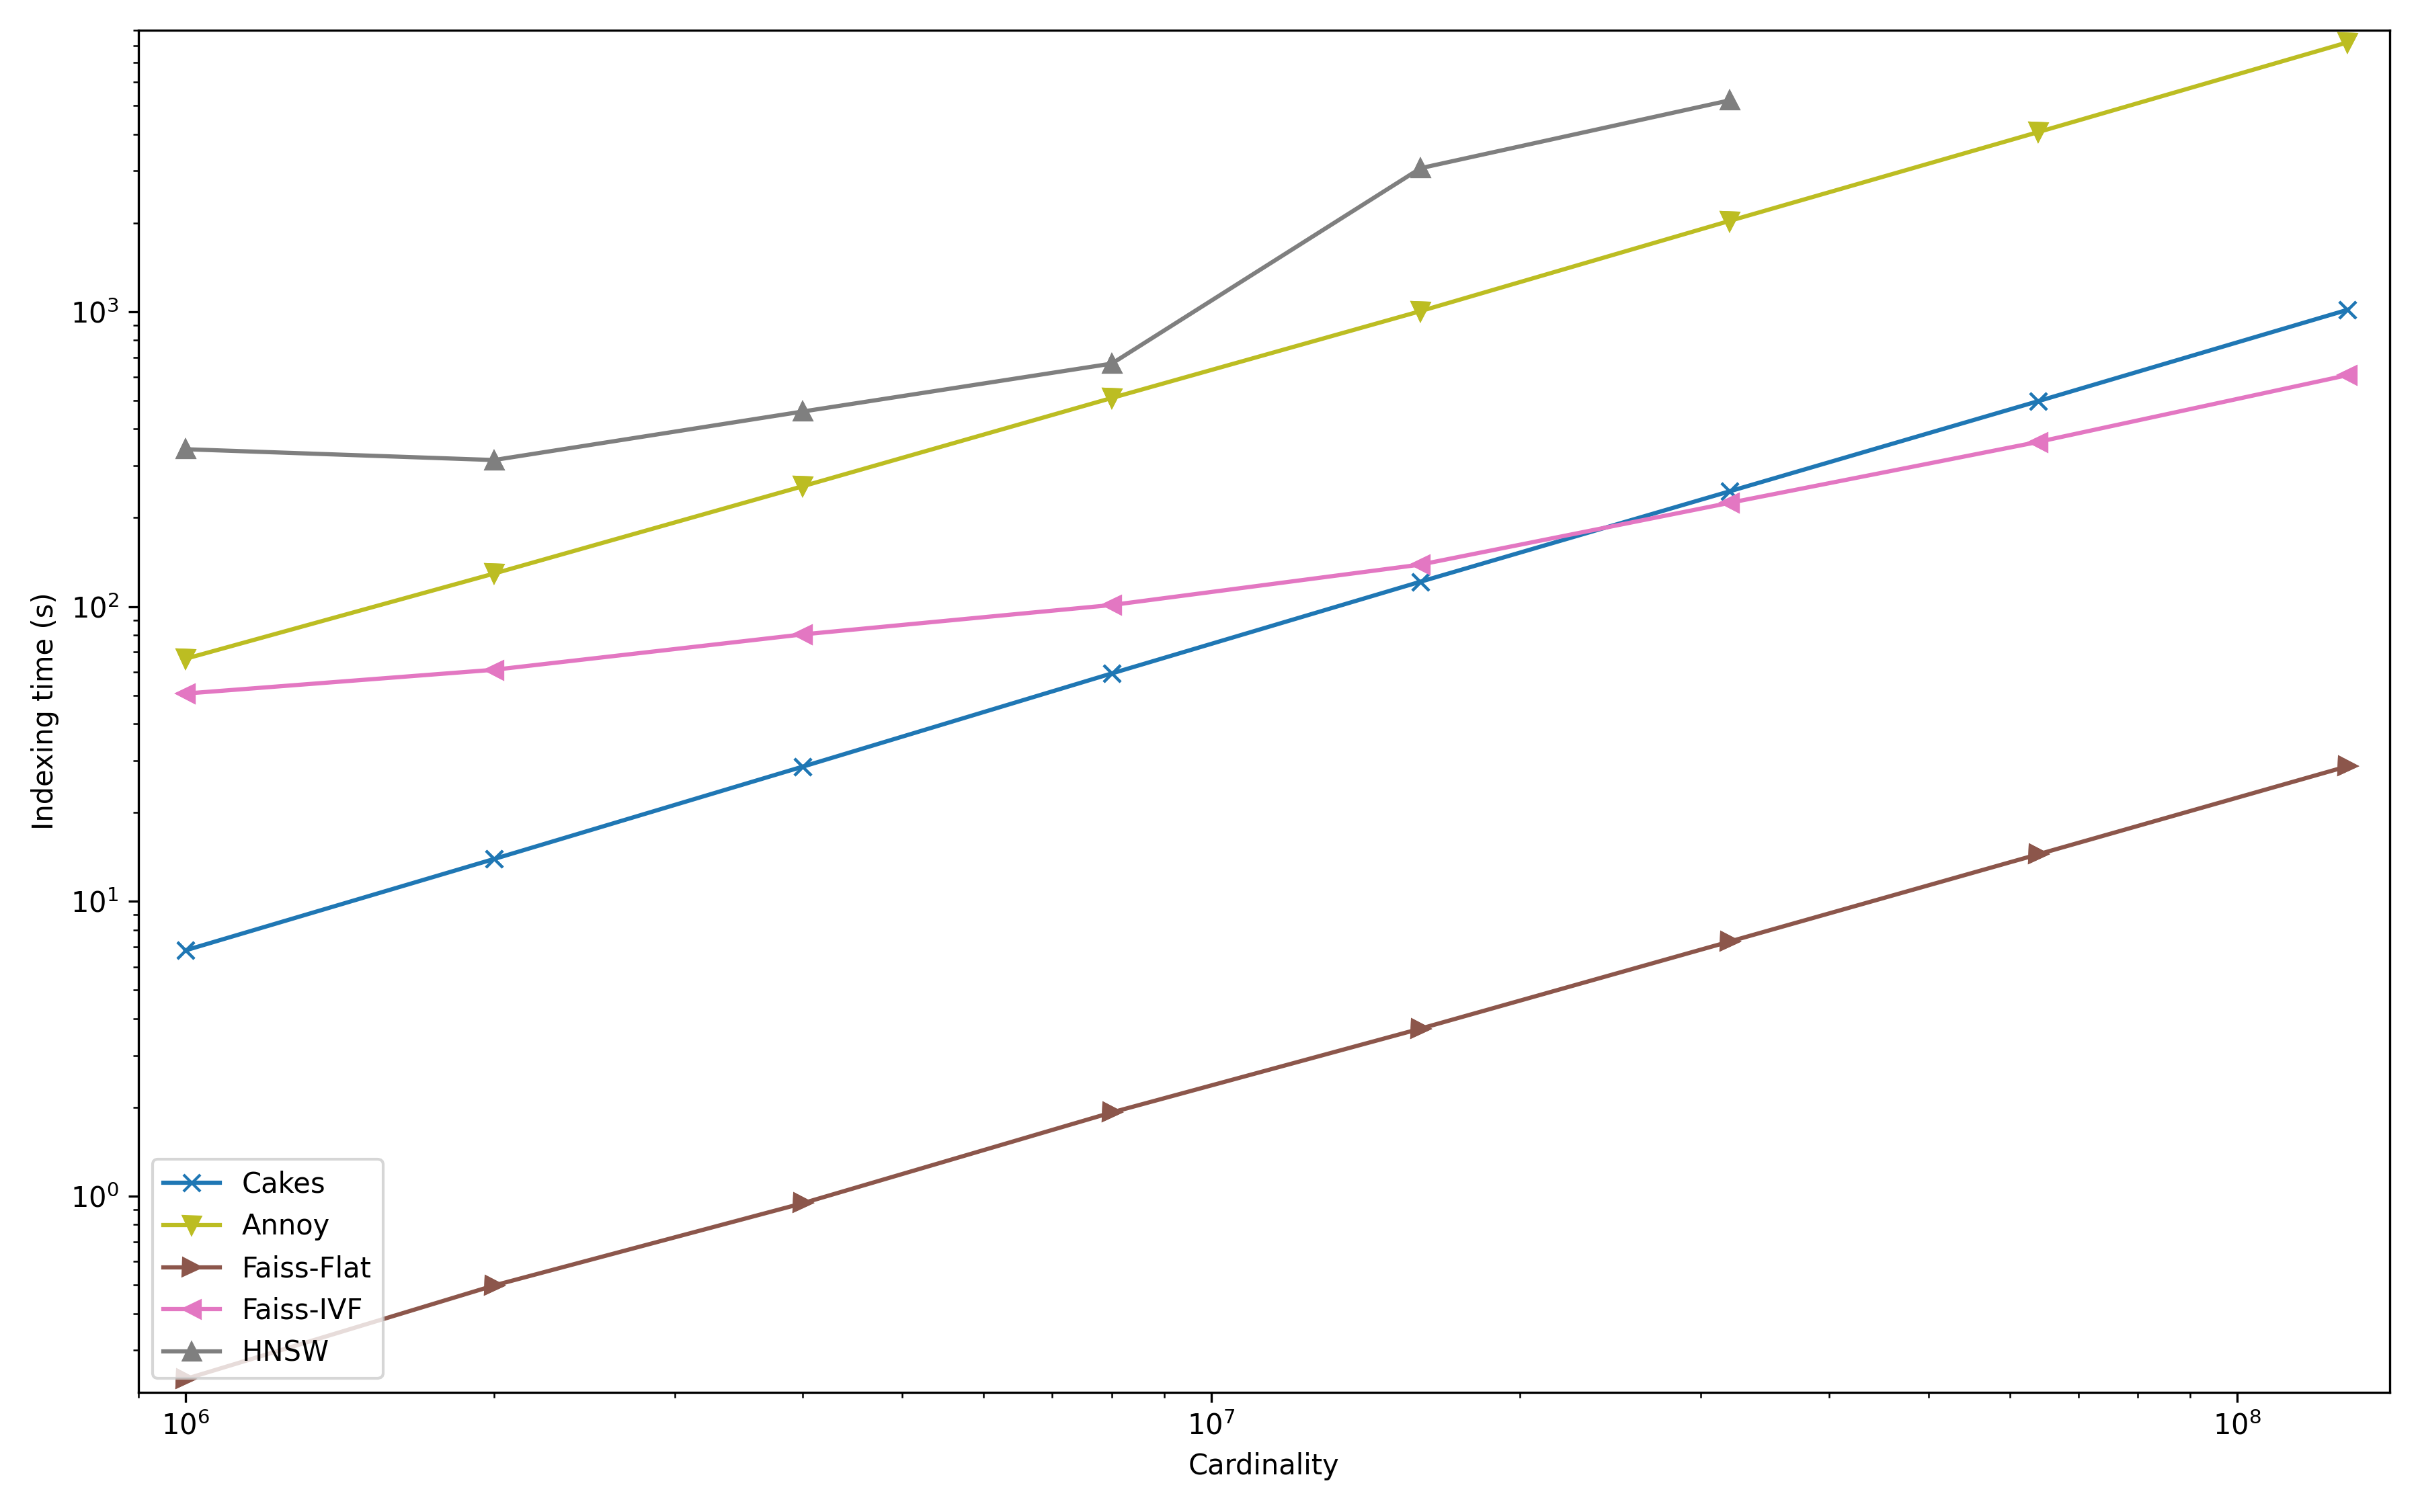
\includegraphics[width=0.95\textwidth]{plots/sift-indexing.png}\\
        \subcaption{Sift}
        \label{fig:supplement:sift-indexing}
    \end{subfigure}%
    \begin{subfigure}[b]{0.47\textwidth}
        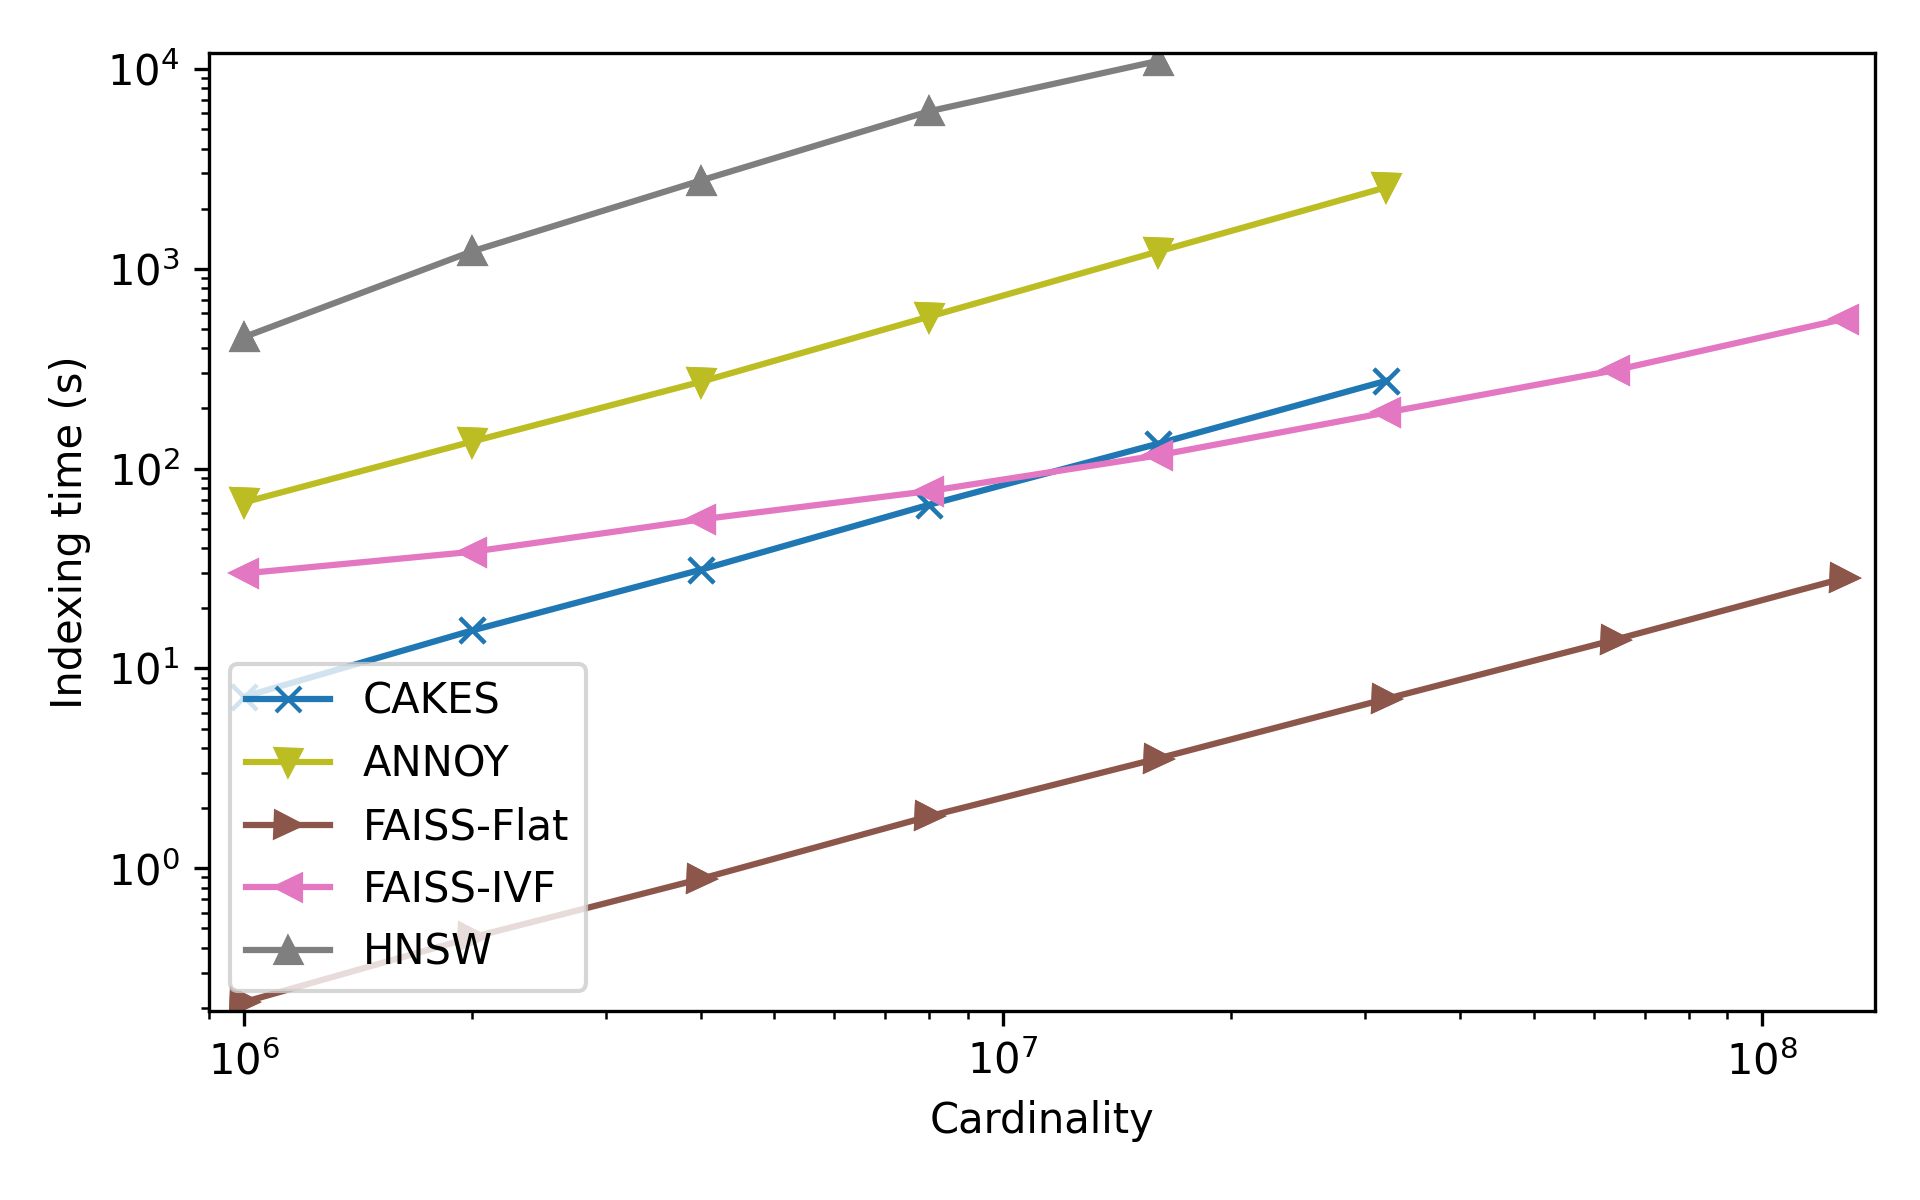
\includegraphics[width=0.95\textwidth]{plots/random-indexing.png}\\
        \subcaption{Random}
        \label{fig:supplement:random-indexing}
    \end{subfigure}%
    \\
    \vspace{1em}
    \caption{Indexing and tuning time for each algorithm with each of the ANN benchmark datasets and the Random dataset.}
    \label{fig:supplement:indexing}
\end{figure}

\begin{figure}[ht!]
    \centering
    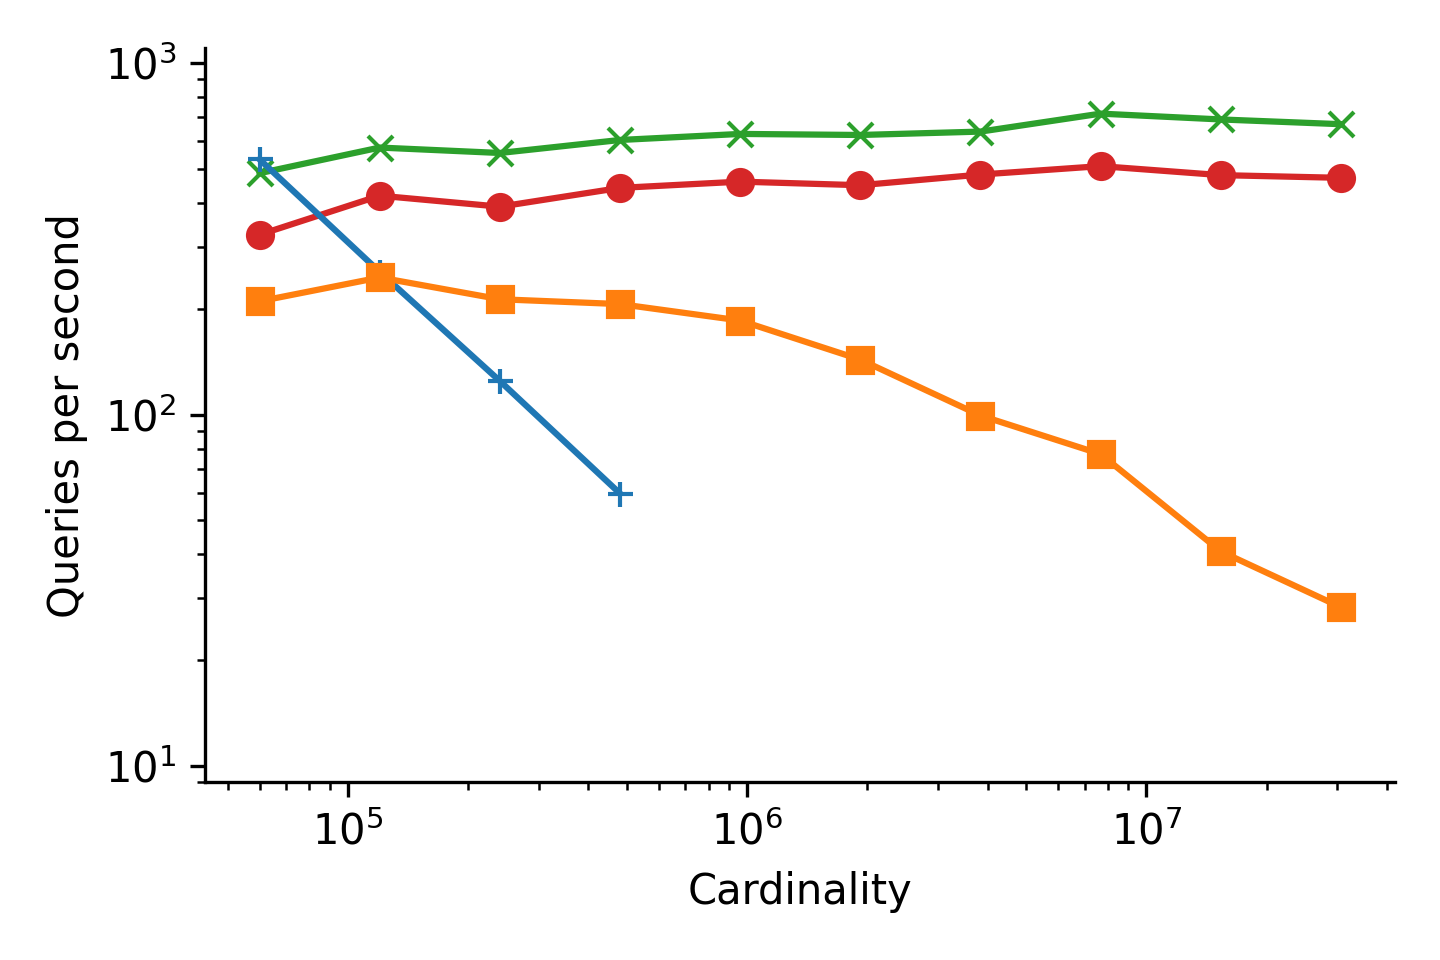
\includegraphics[width=3.4in]{plots/fashion-mnist_PermutedBall_100_throughput.png}
    \caption{
        Scaling behavior of algorithms on fashion-mnist with $k=100$.
    }
    \label{fig:supplement:fashion-mnist-k-100}
\end{figure}

\begin{figure}[ht!]
    \centering
    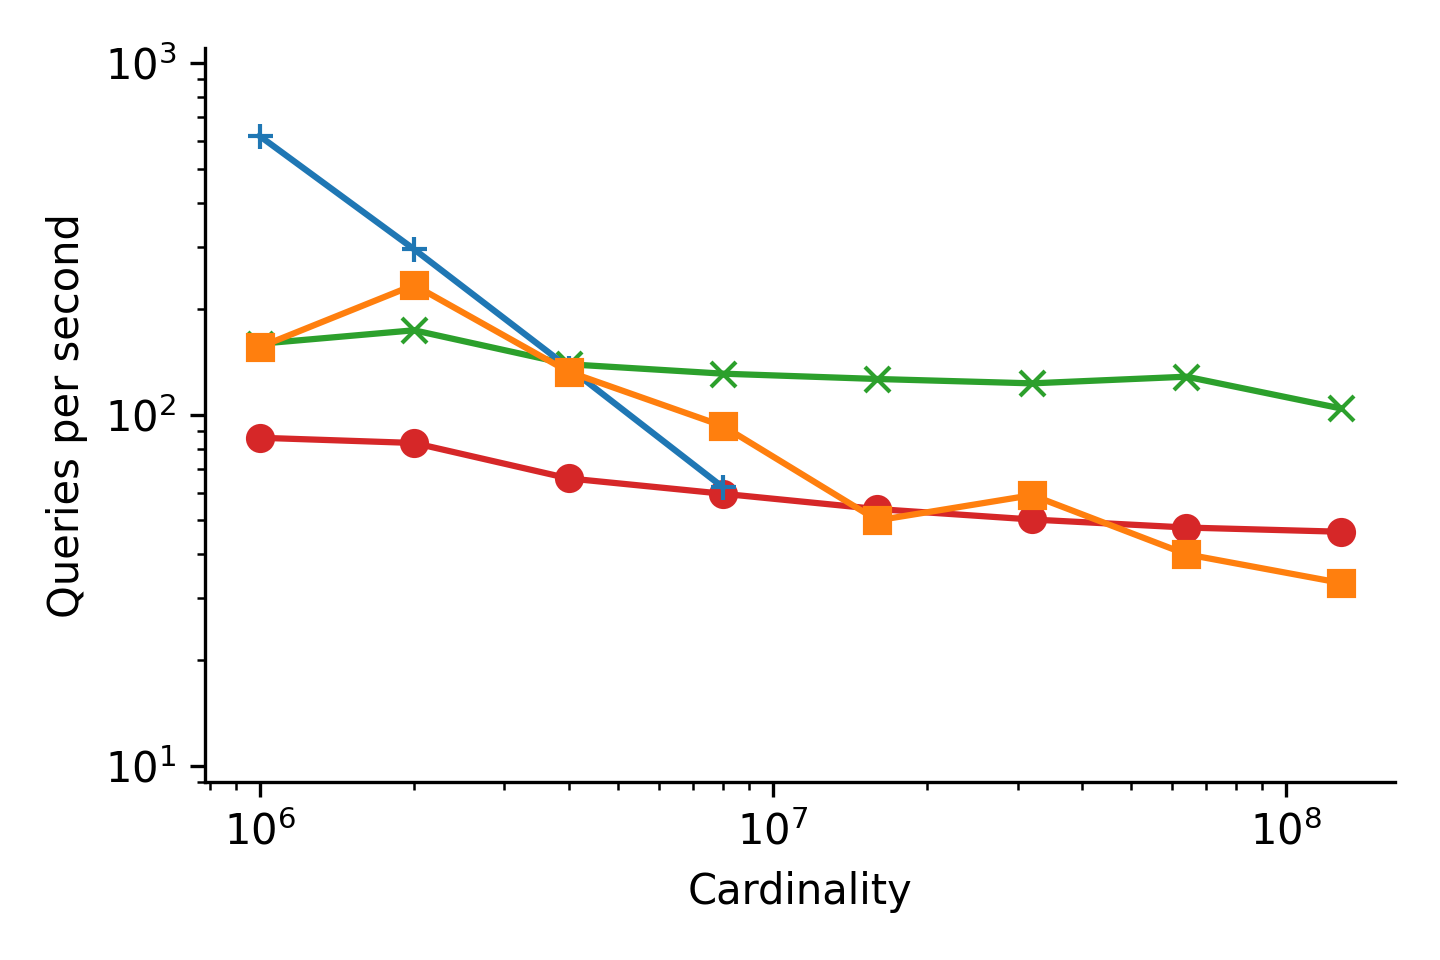
\includegraphics[width=3.4in]{plots/sift_PermutedBall_100_throughput.png}
    \caption{
        Scaling behavior of algorithms on sift with $k=100$.
    }
    \label{fig:supplement:sift-k-100}
\end{figure}

\begin{figure}[ht!]
    \centering
    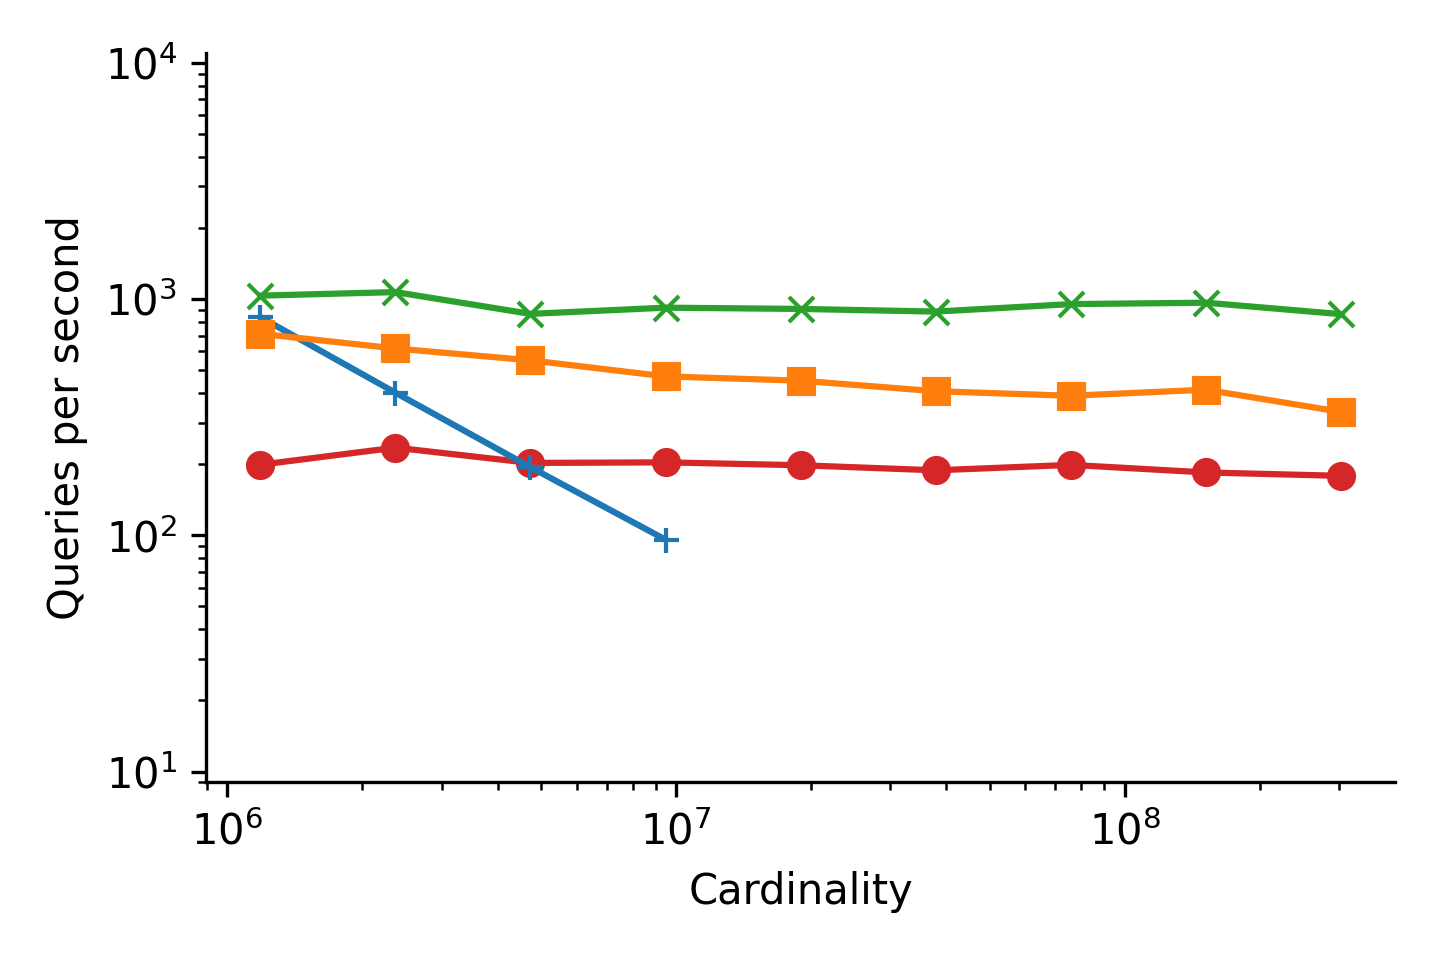
\includegraphics[width=3.4in]{plots/glove-25_PermutedBall_100_throughput.png}
    \caption{
        Scaling behavior of algorithms on glove-25 with $k=100$.
    }
    \label{fig:supplement:glove-25-k-100}
\end{figure}

\begin{figure}[ht!]
    \centering
    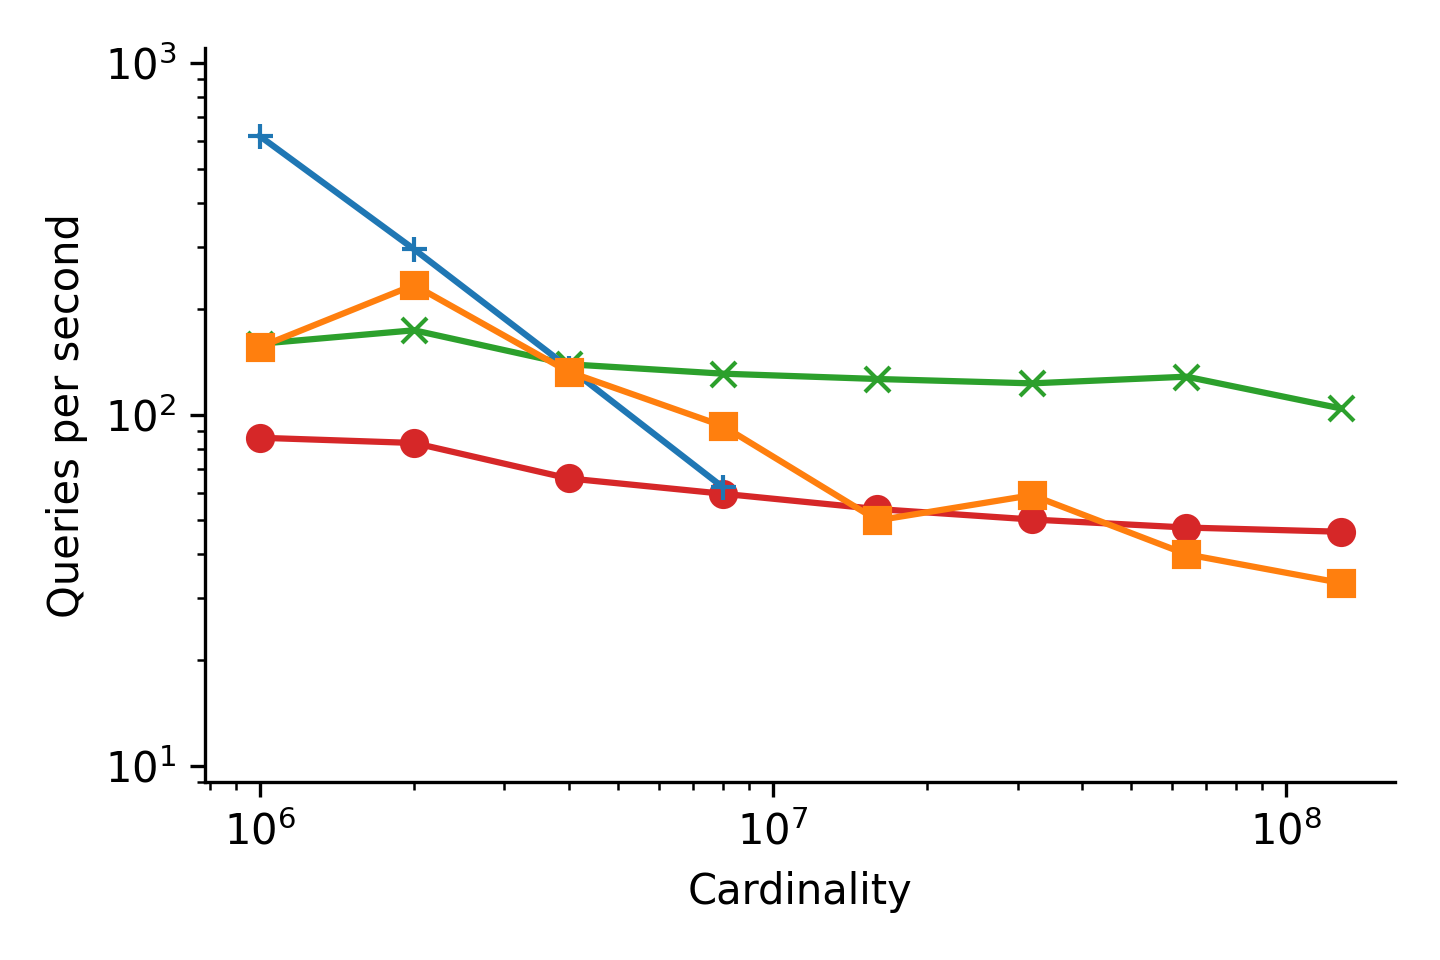
\includegraphics[width=3.4in]{plots/sift_PermutedBall_100_throughput.png}
    \caption{
        Scaling behavior of algorithms on random with $k=100$.
    }
    \label{fig:supplement:random-k-100}
\end{figure}

\subsection{Clustering}

\begin{figure}[ht!]
    \begin{subfigure}[b]{0.47\textwidth}
    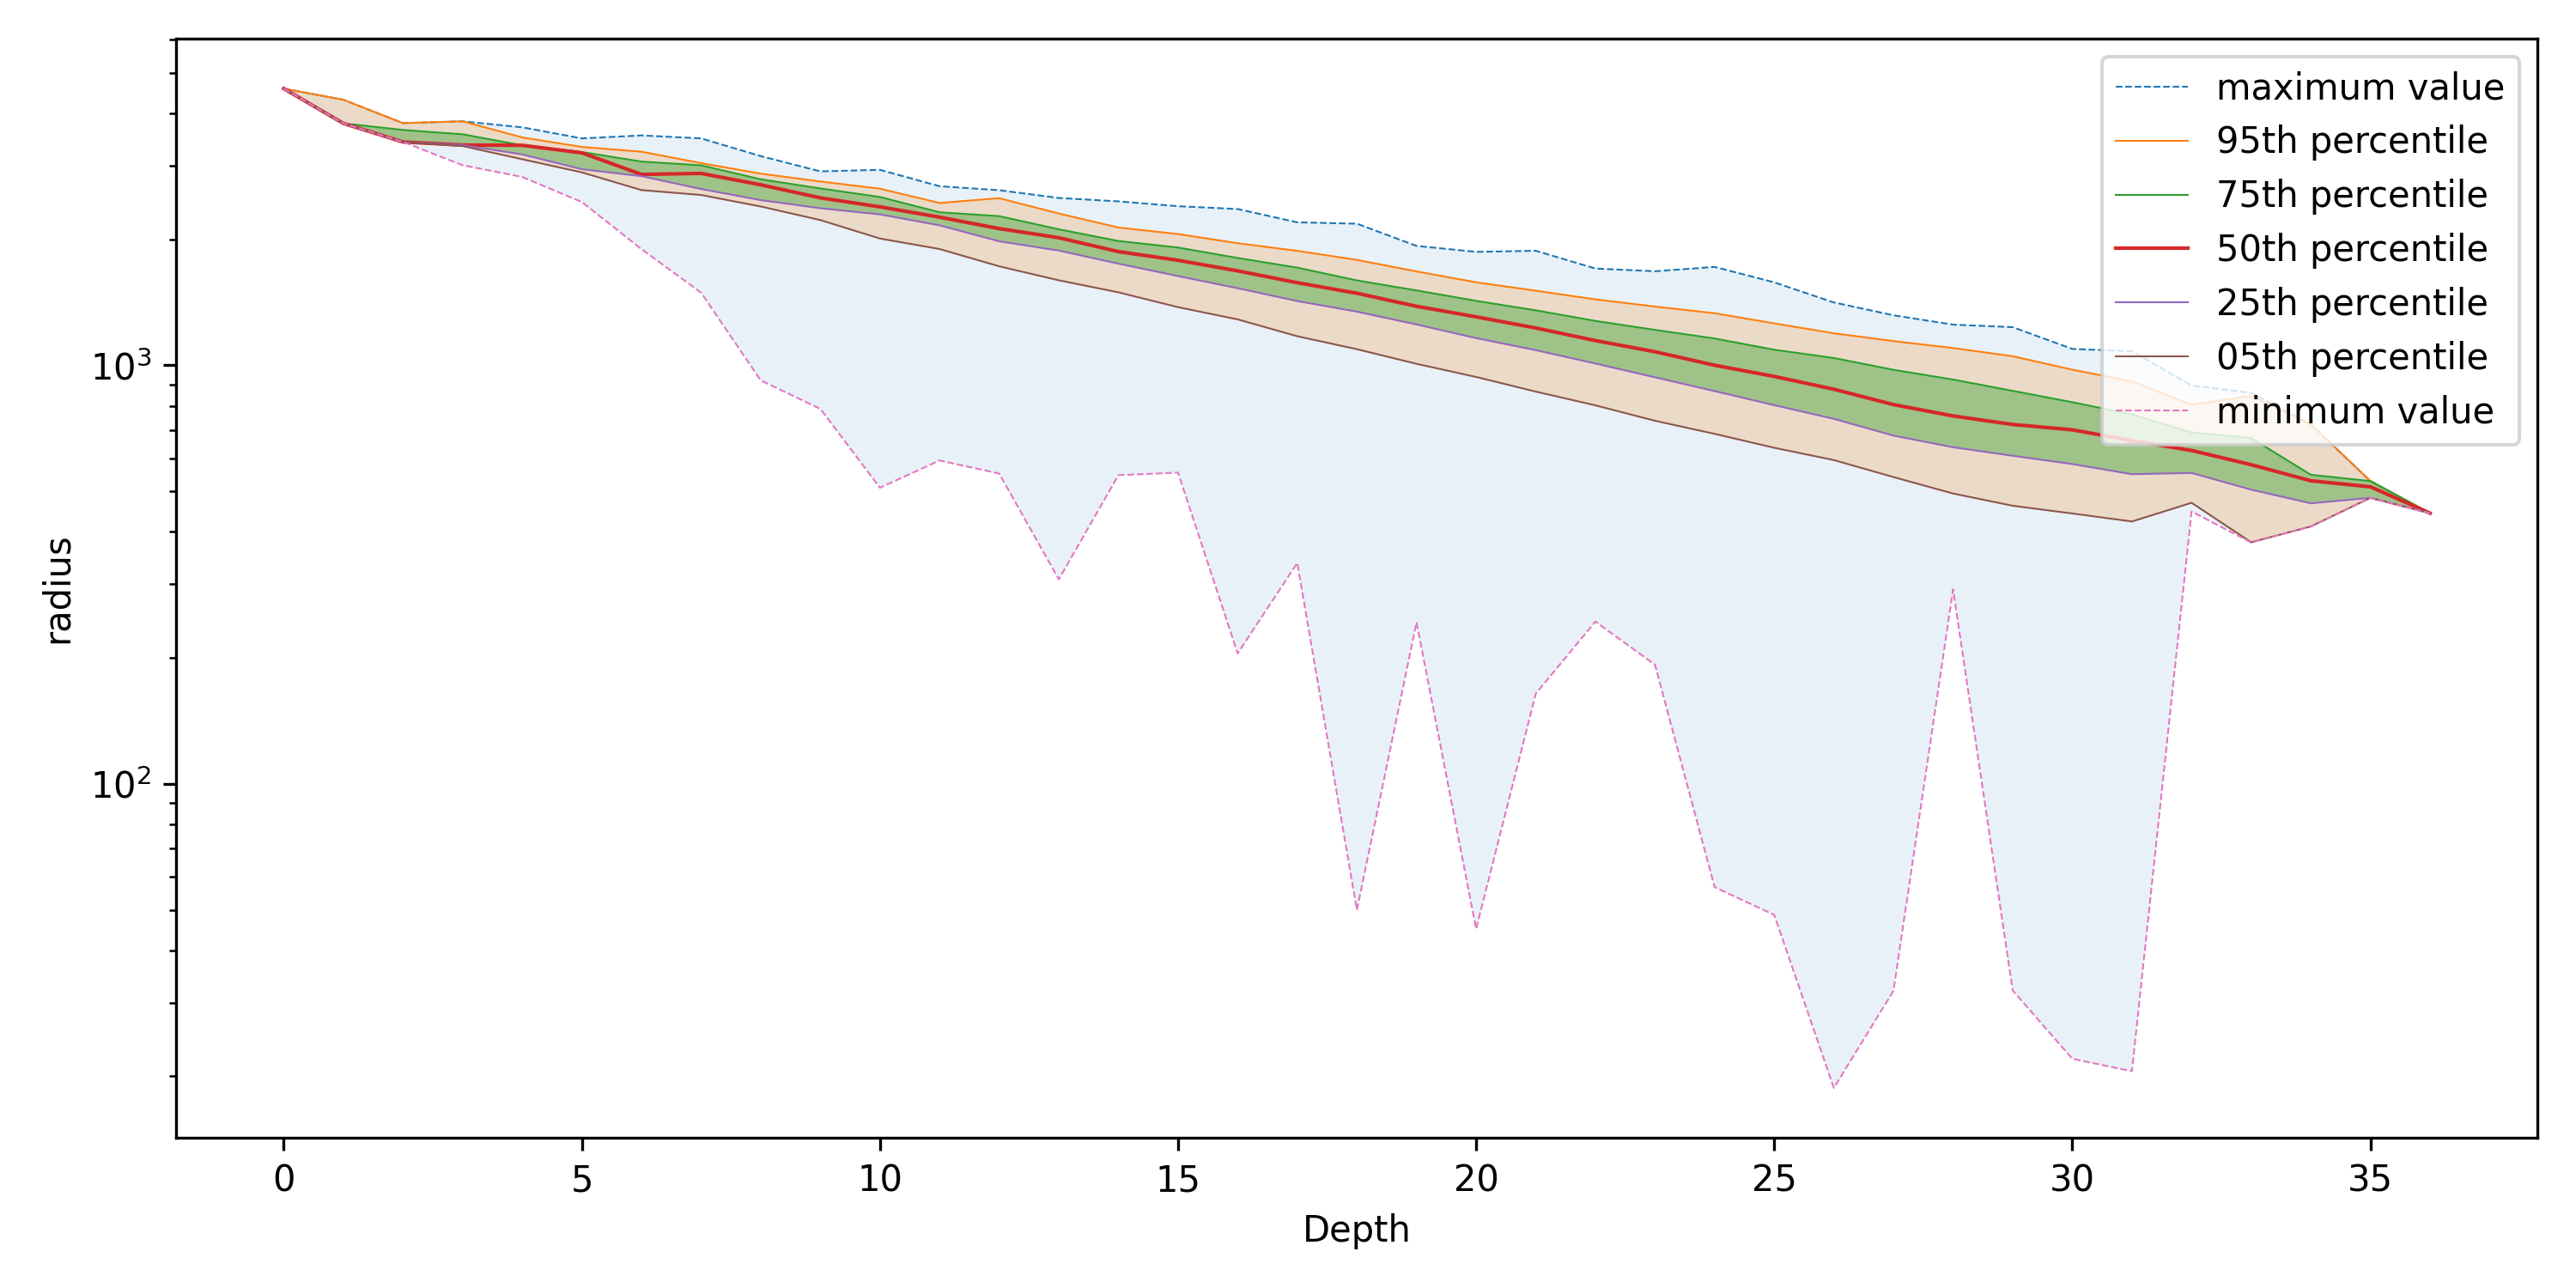
\includegraphics[width=0.95\textwidth]{images/radius/fashion-mnist-60000.png}\\
    \subcaption{Fashion-mnist}
    \label{fig:results:fashion-mnist-radius}
    \end{subfigure}%
    \begin{subfigure}[b]{0.47\textwidth}
    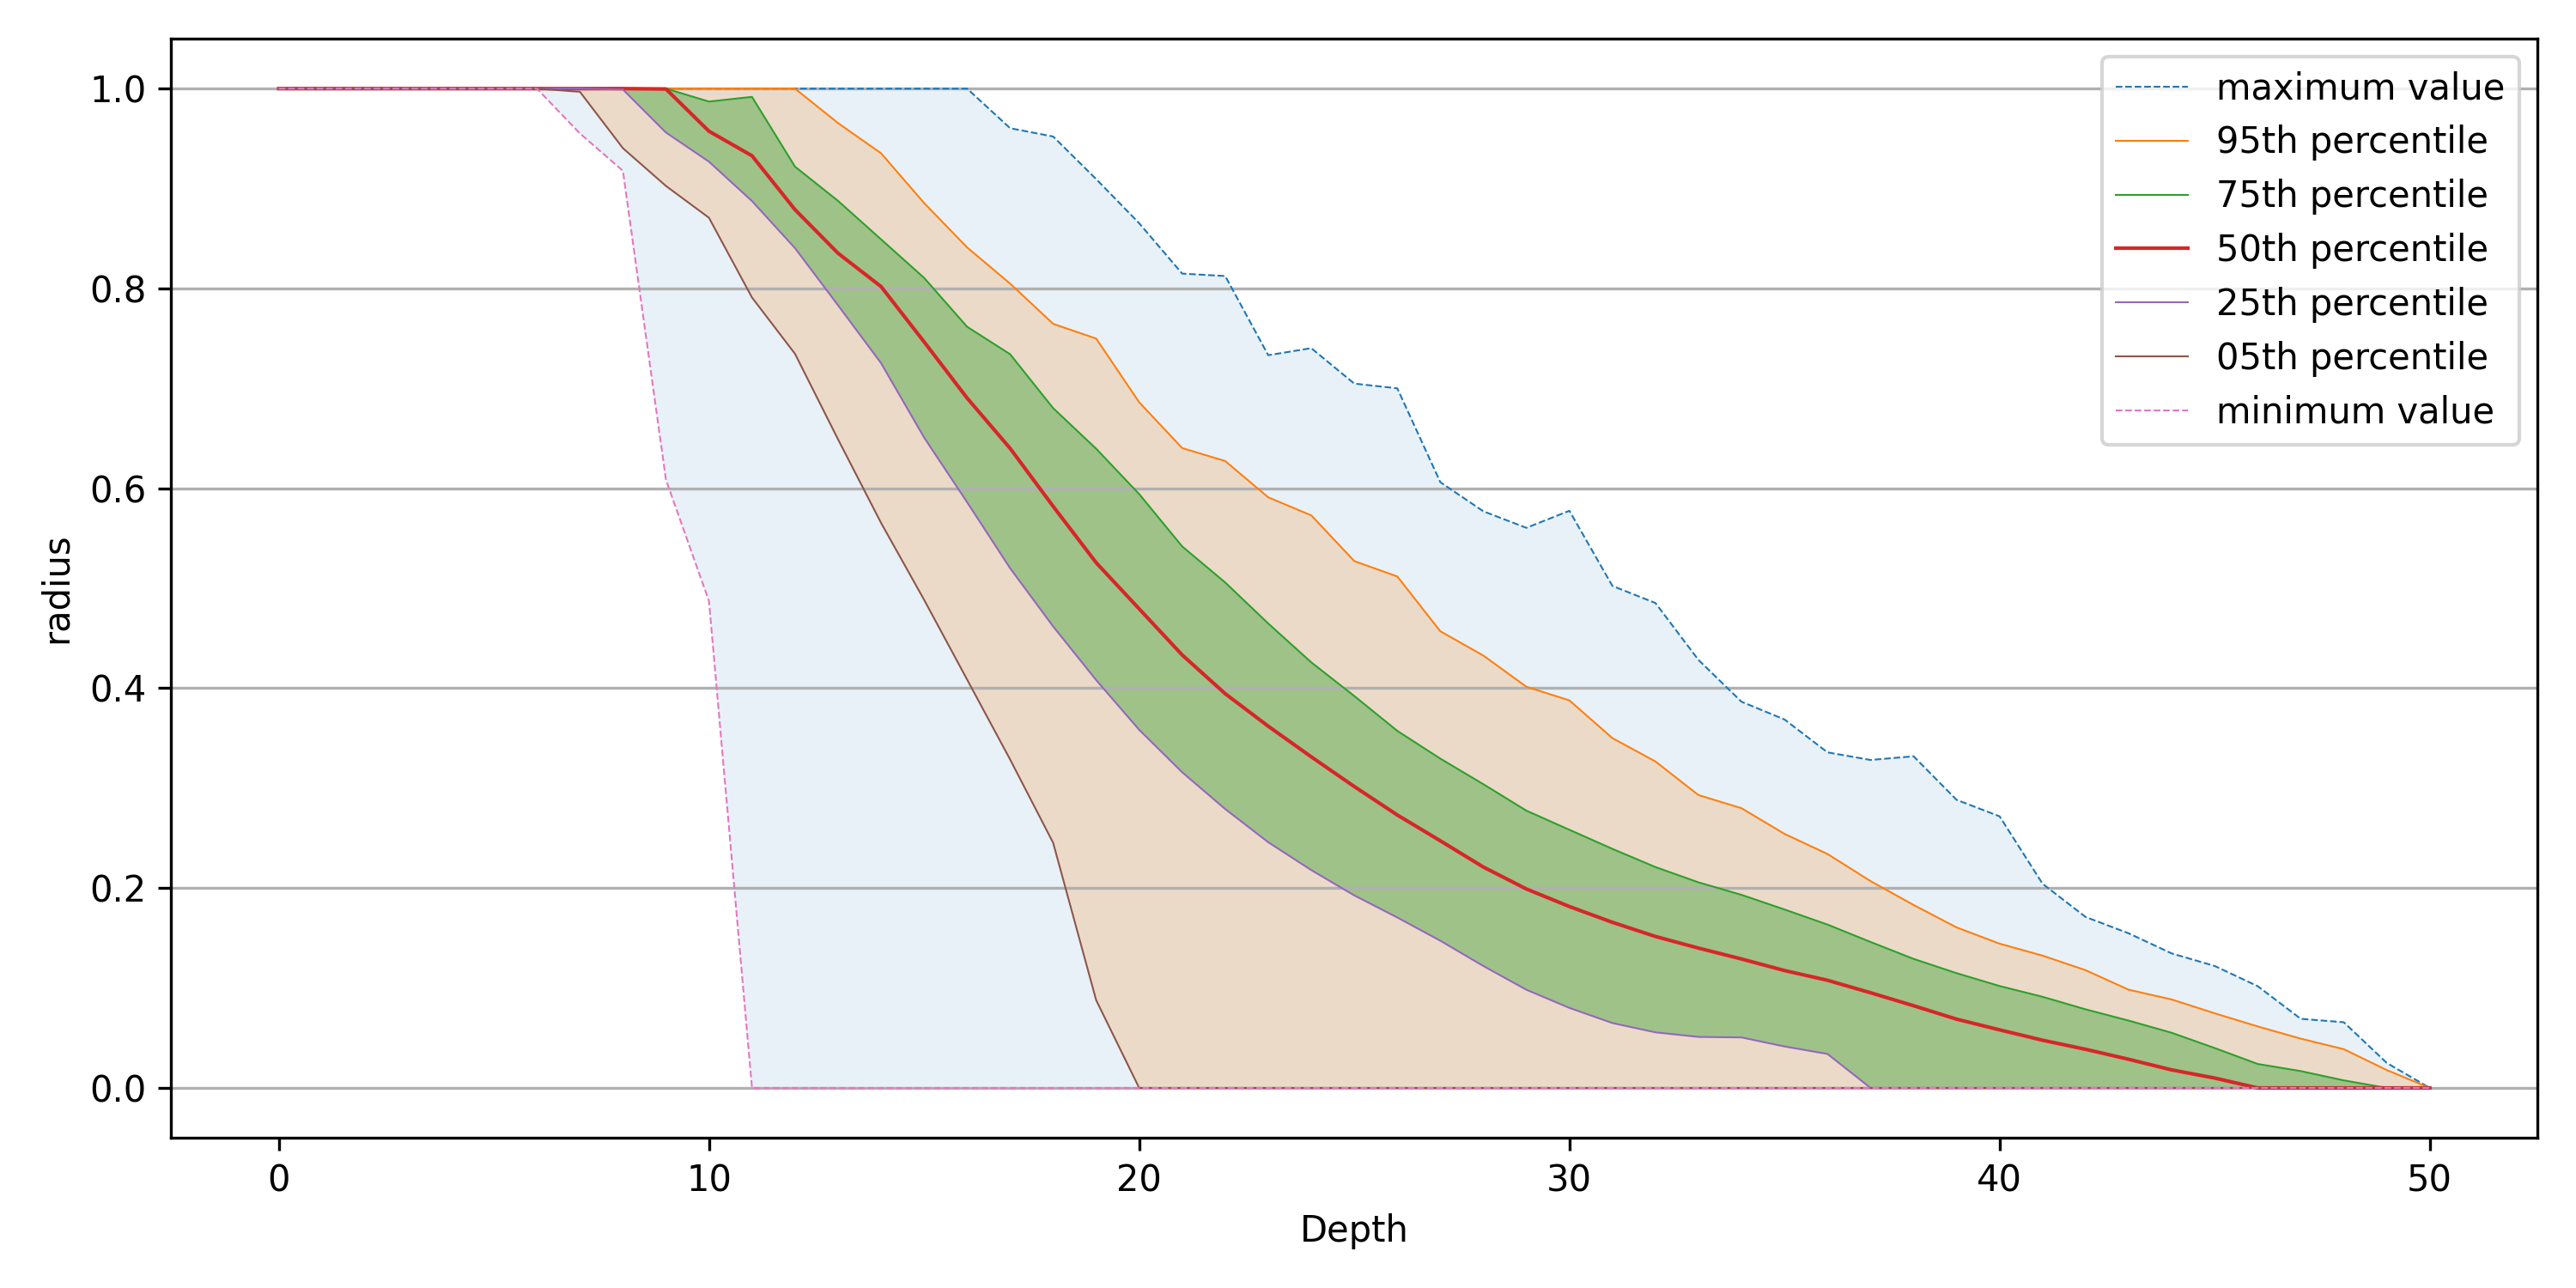
\includegraphics[width=0.95\textwidth]{images/radius/glove-25-1183514.png}\\
    \subcaption{Glove-25}
    \label{fig:results:glove-25-radius}
    \end{subfigure}
    \vspace{1em}
    \\
    \begin{subfigure}[b]{0.47\textwidth}
    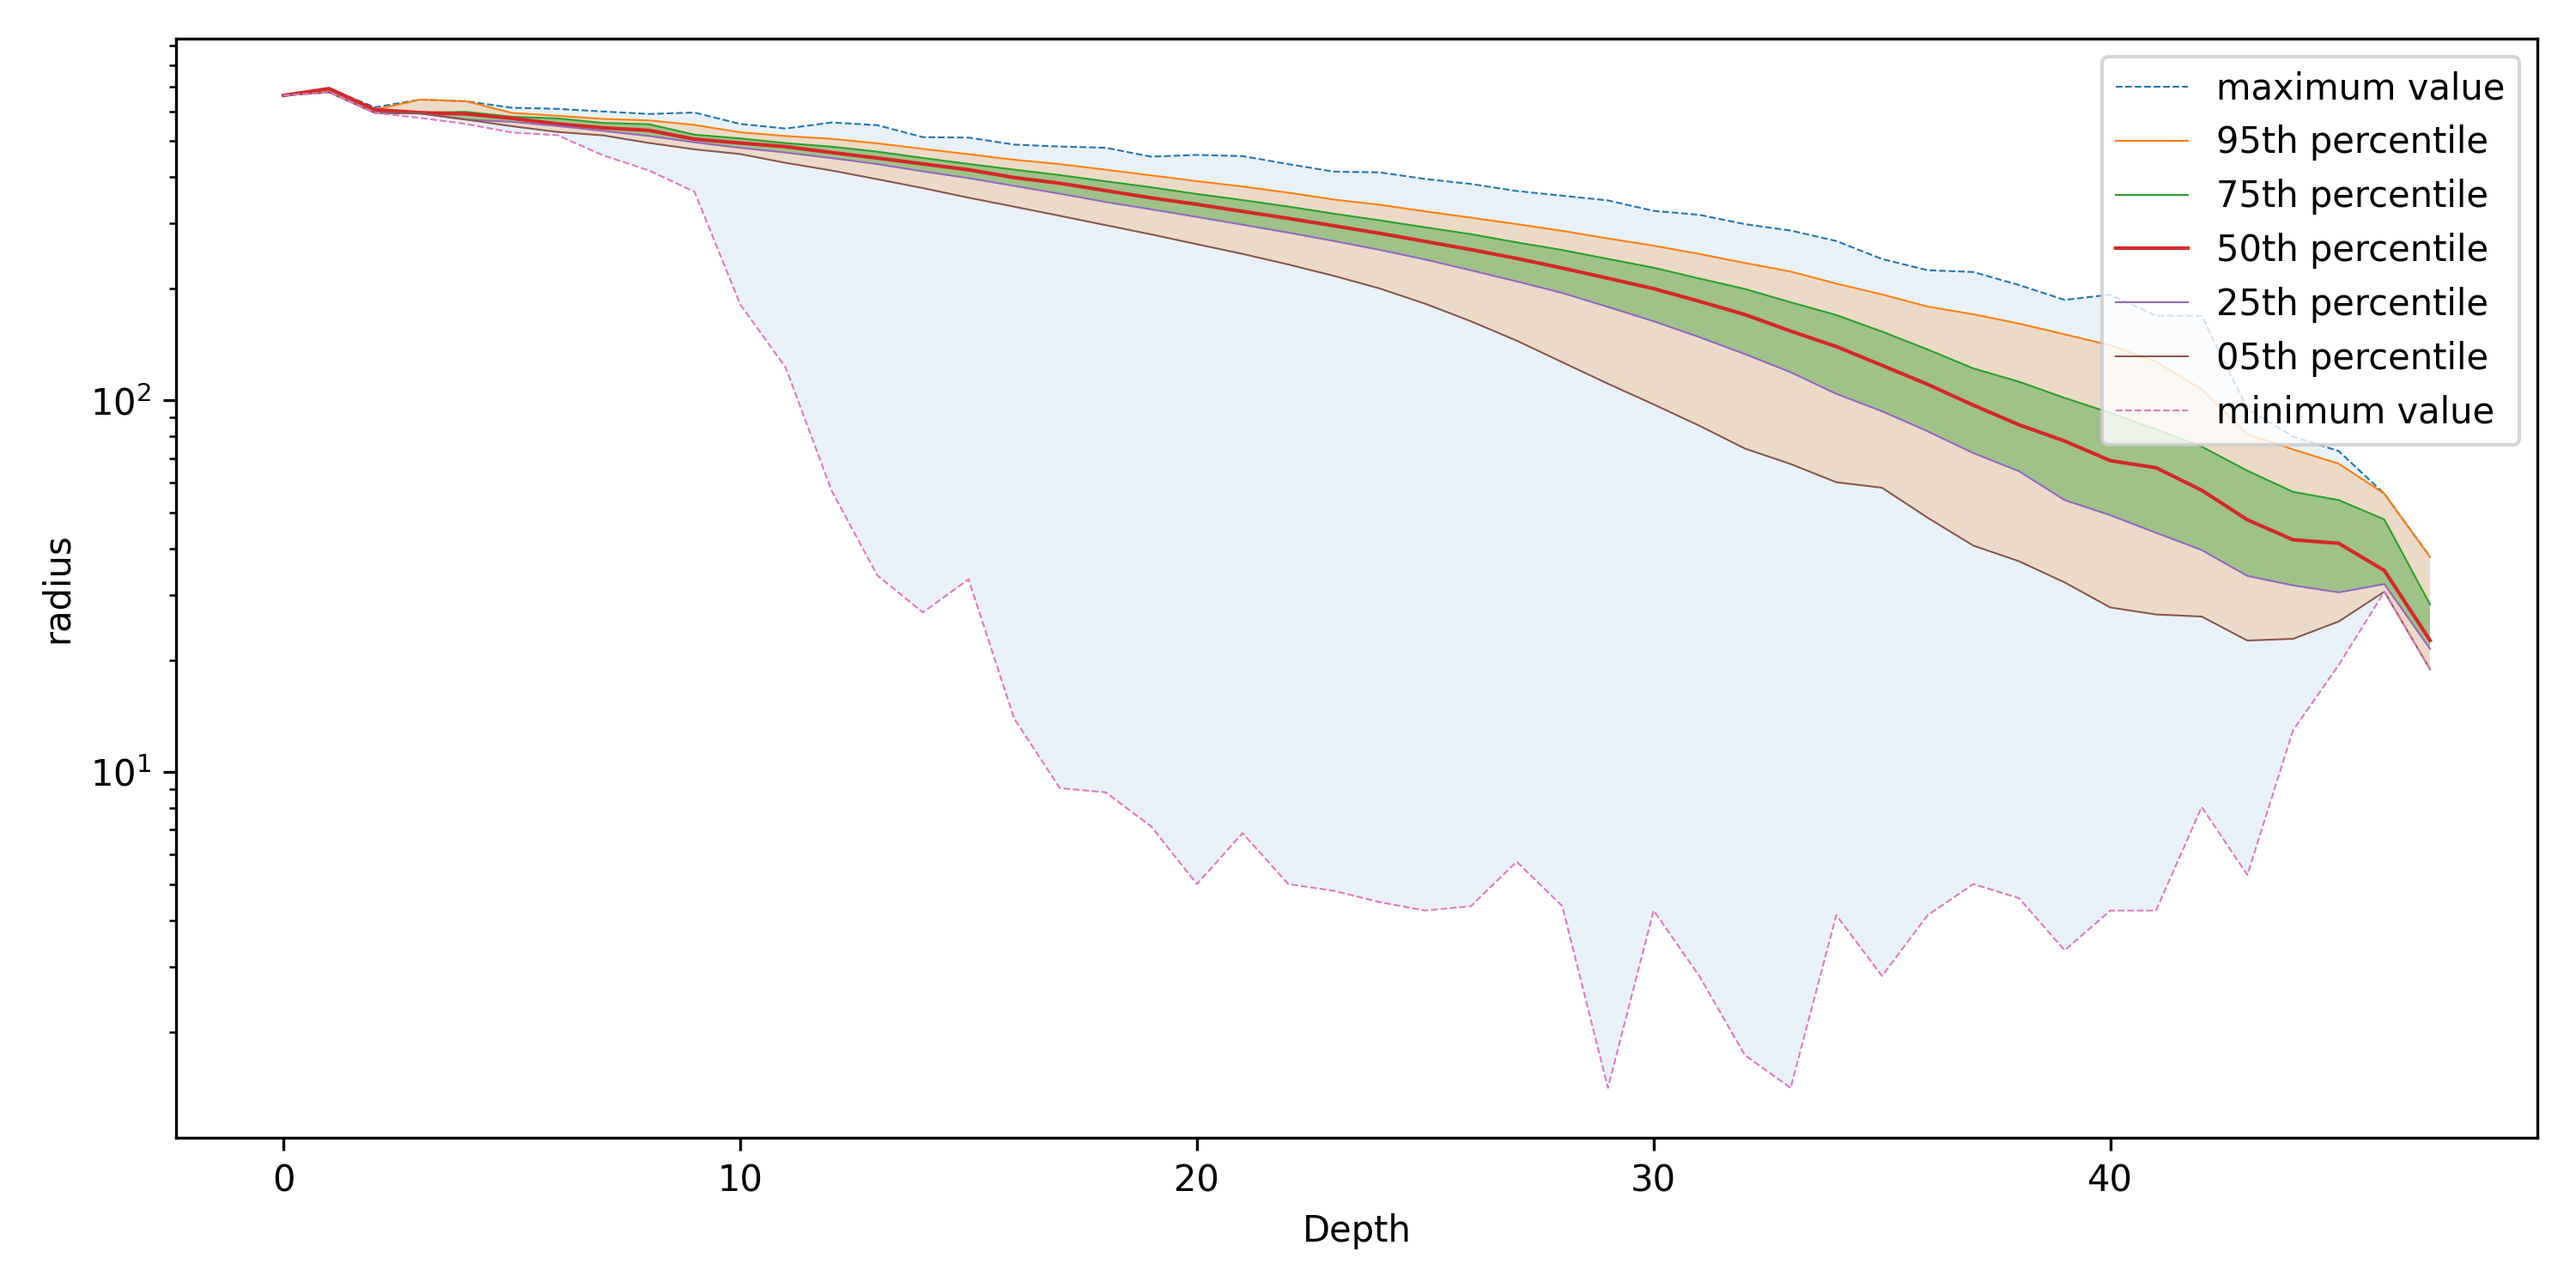
\includegraphics[width=0.95\textwidth]{images/radius/sift-1000000.png}\\
    \subcaption{Sift}
    \label{fig:results:sift-radius}
    \end{subfigure}%
    \begin{subfigure}[b]{0.47\textwidth}
    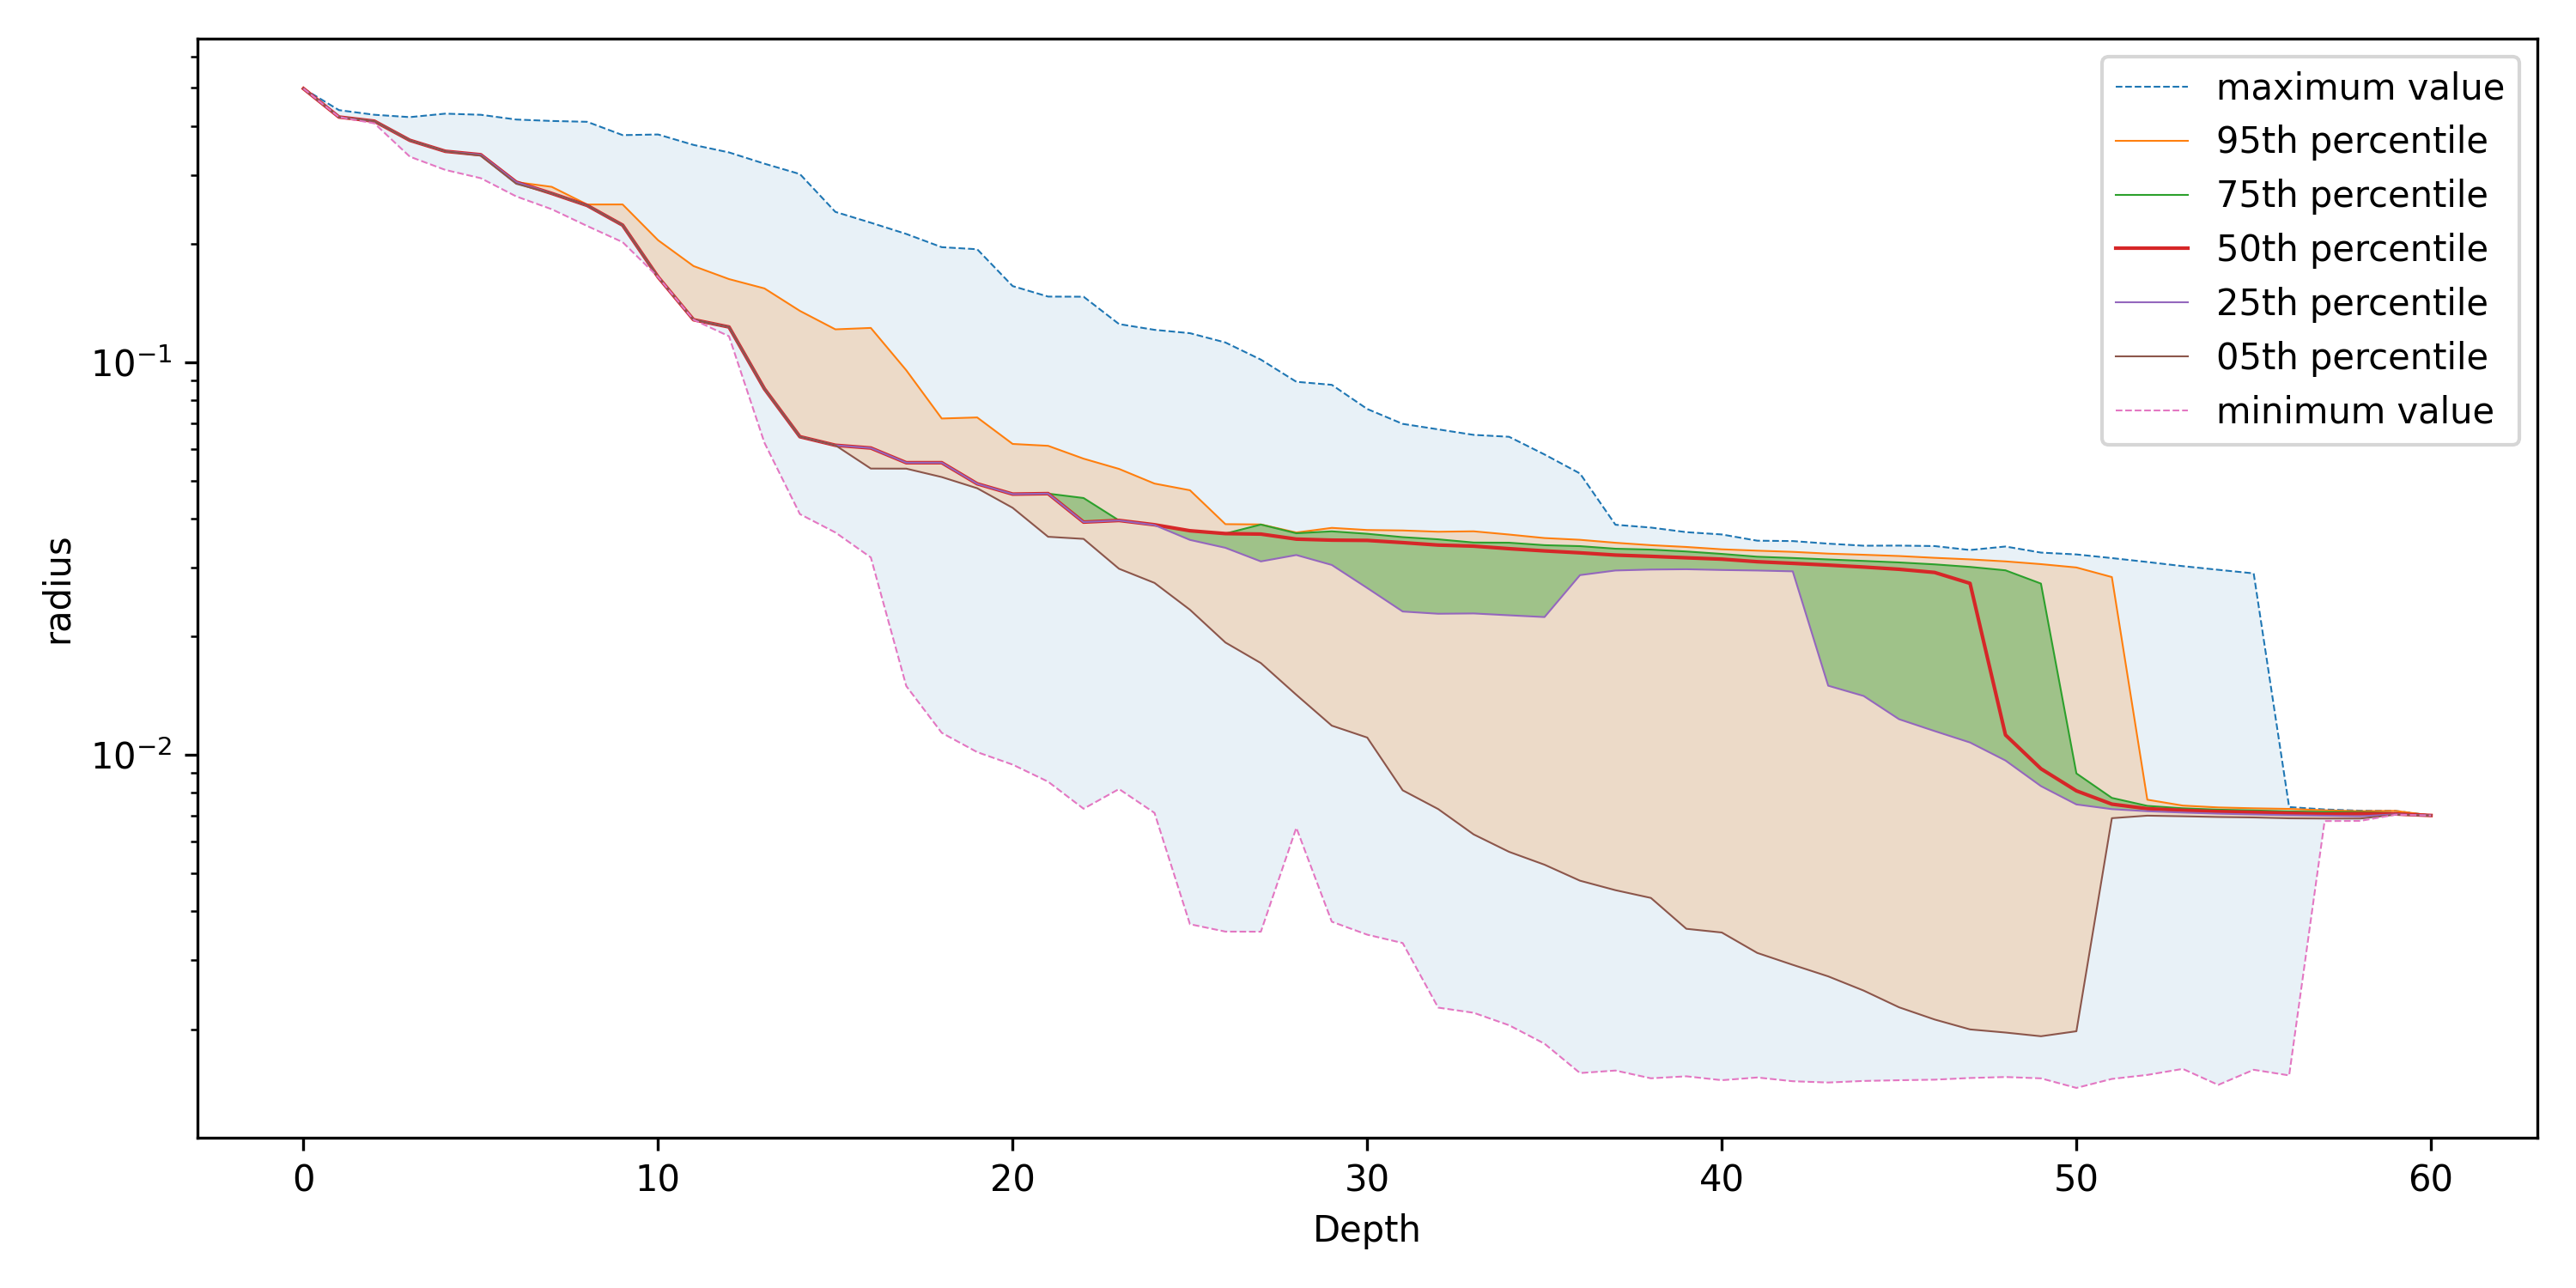
\includegraphics[width=0.95\textwidth]{images/radius/radio-ml-97920.png}\\
    \subcaption{RadioML}
    \label{fig:results:radioml-radius}
    \end{subfigure}%
    \\
    \begin{subfigure}[b]{0.47\textwidth}
    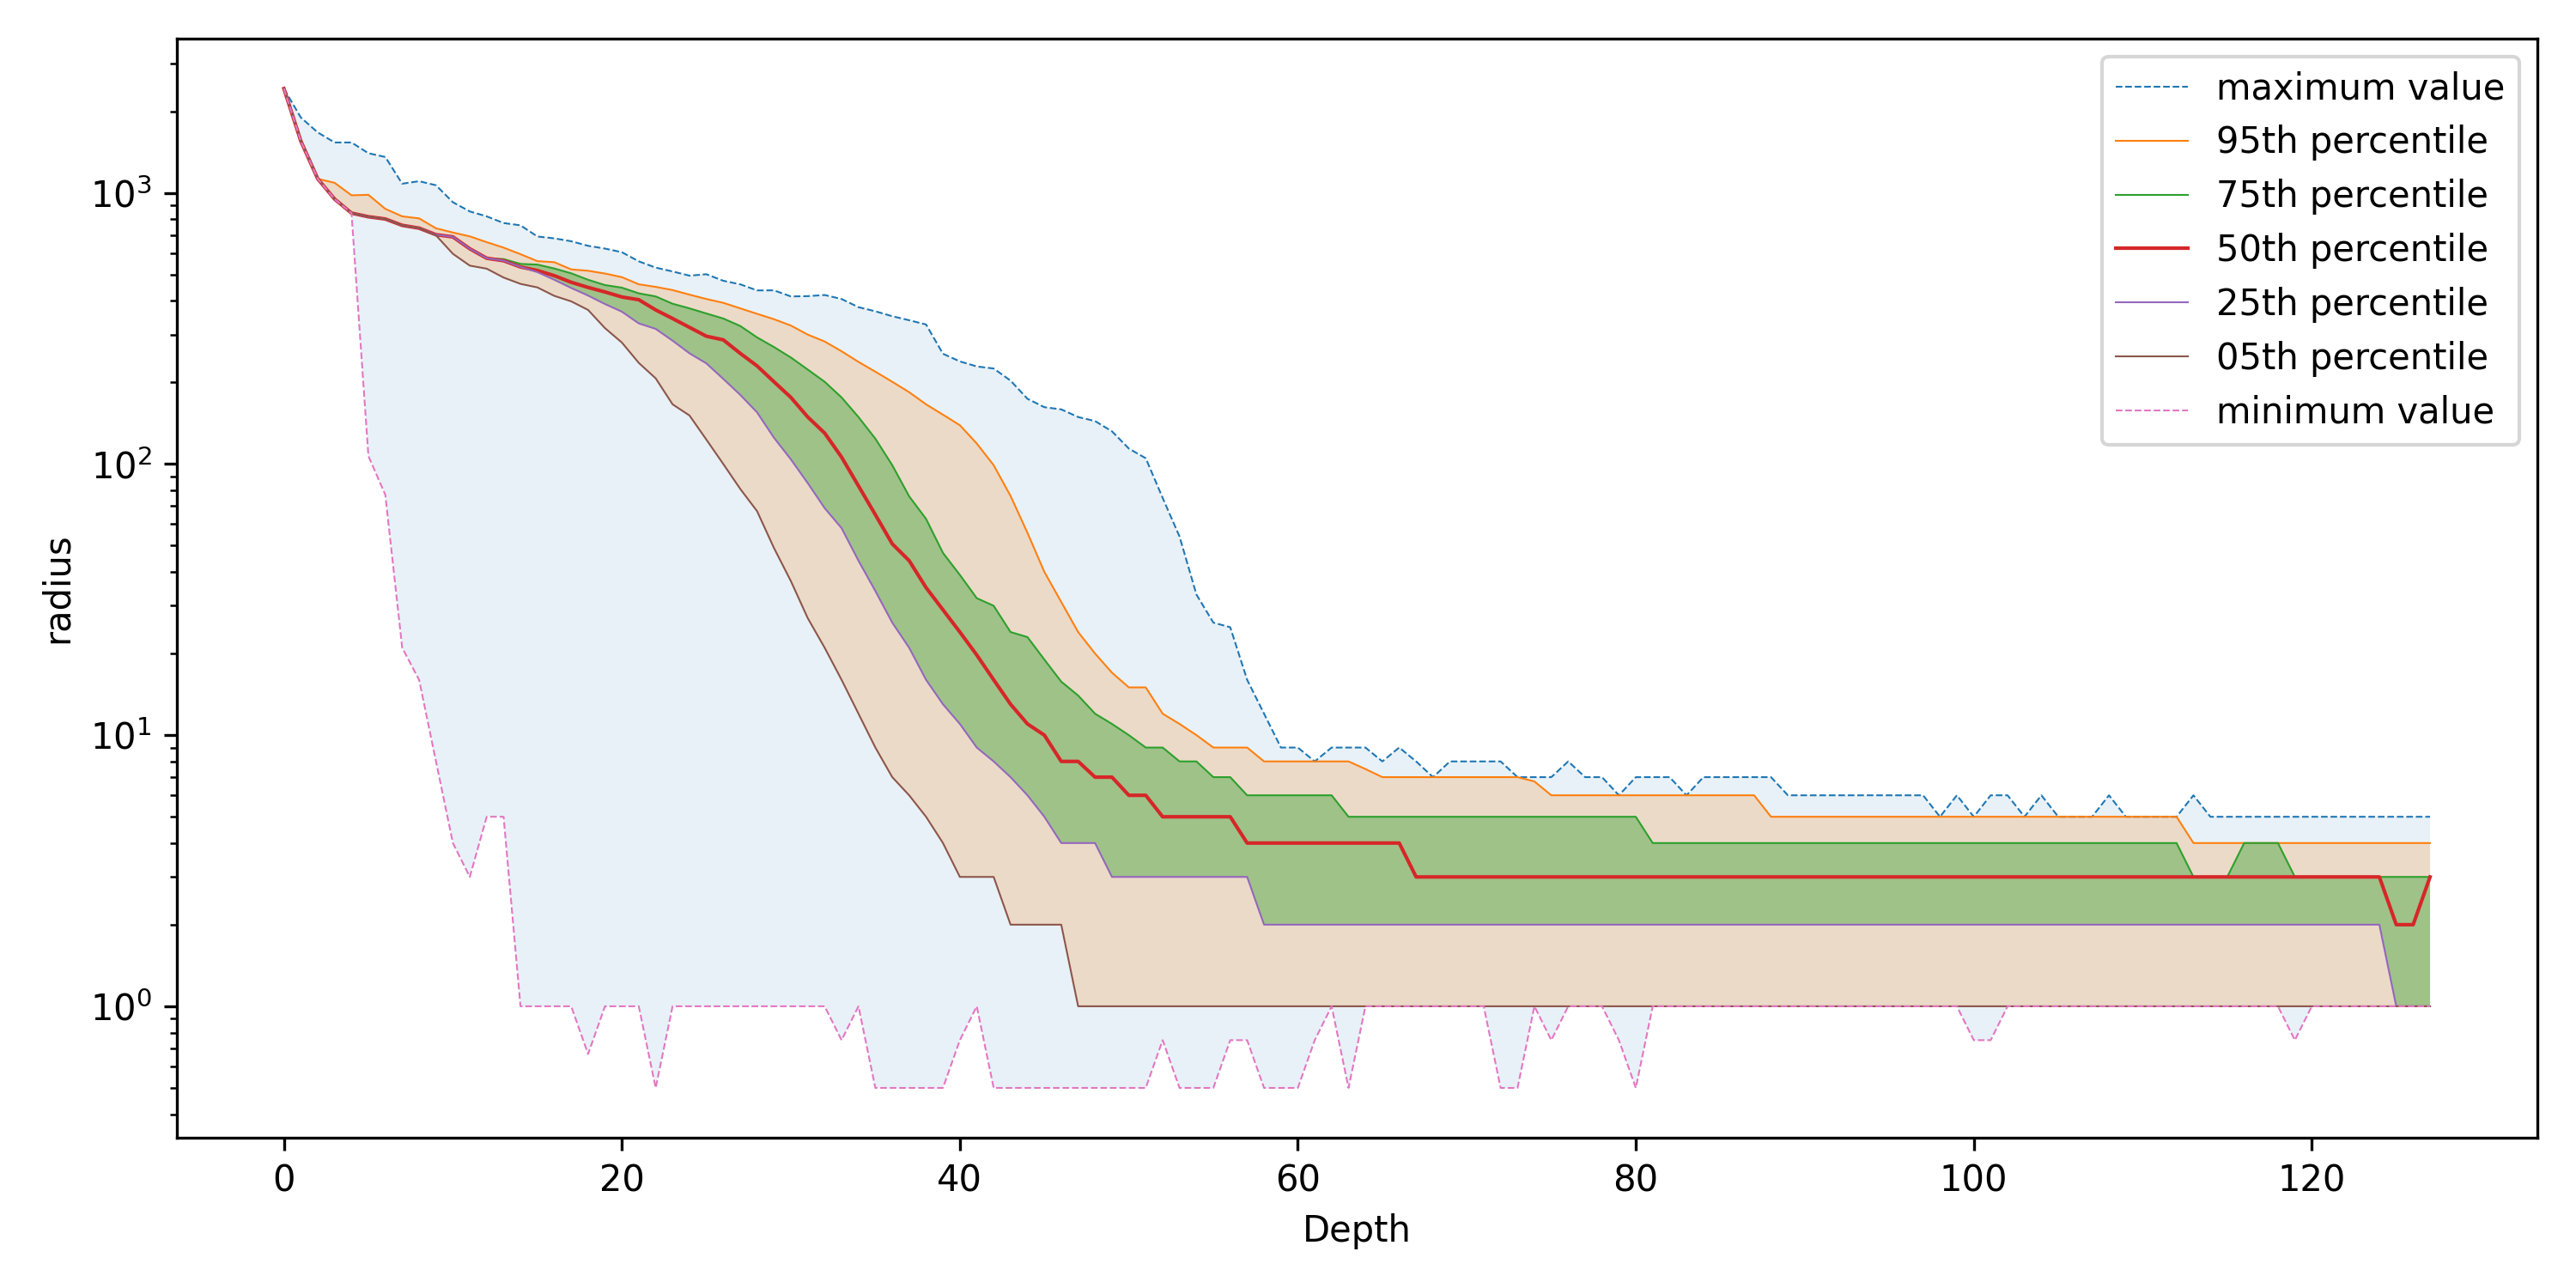
\includegraphics[width=0.95\textwidth]{images/radius/silva-2224640.png}\\
    \subcaption{Silva 18S}
    \label{fig:results:silva-radius}
    \end{subfigure}%
    \begin{subfigure}[b]{0.47\textwidth}
    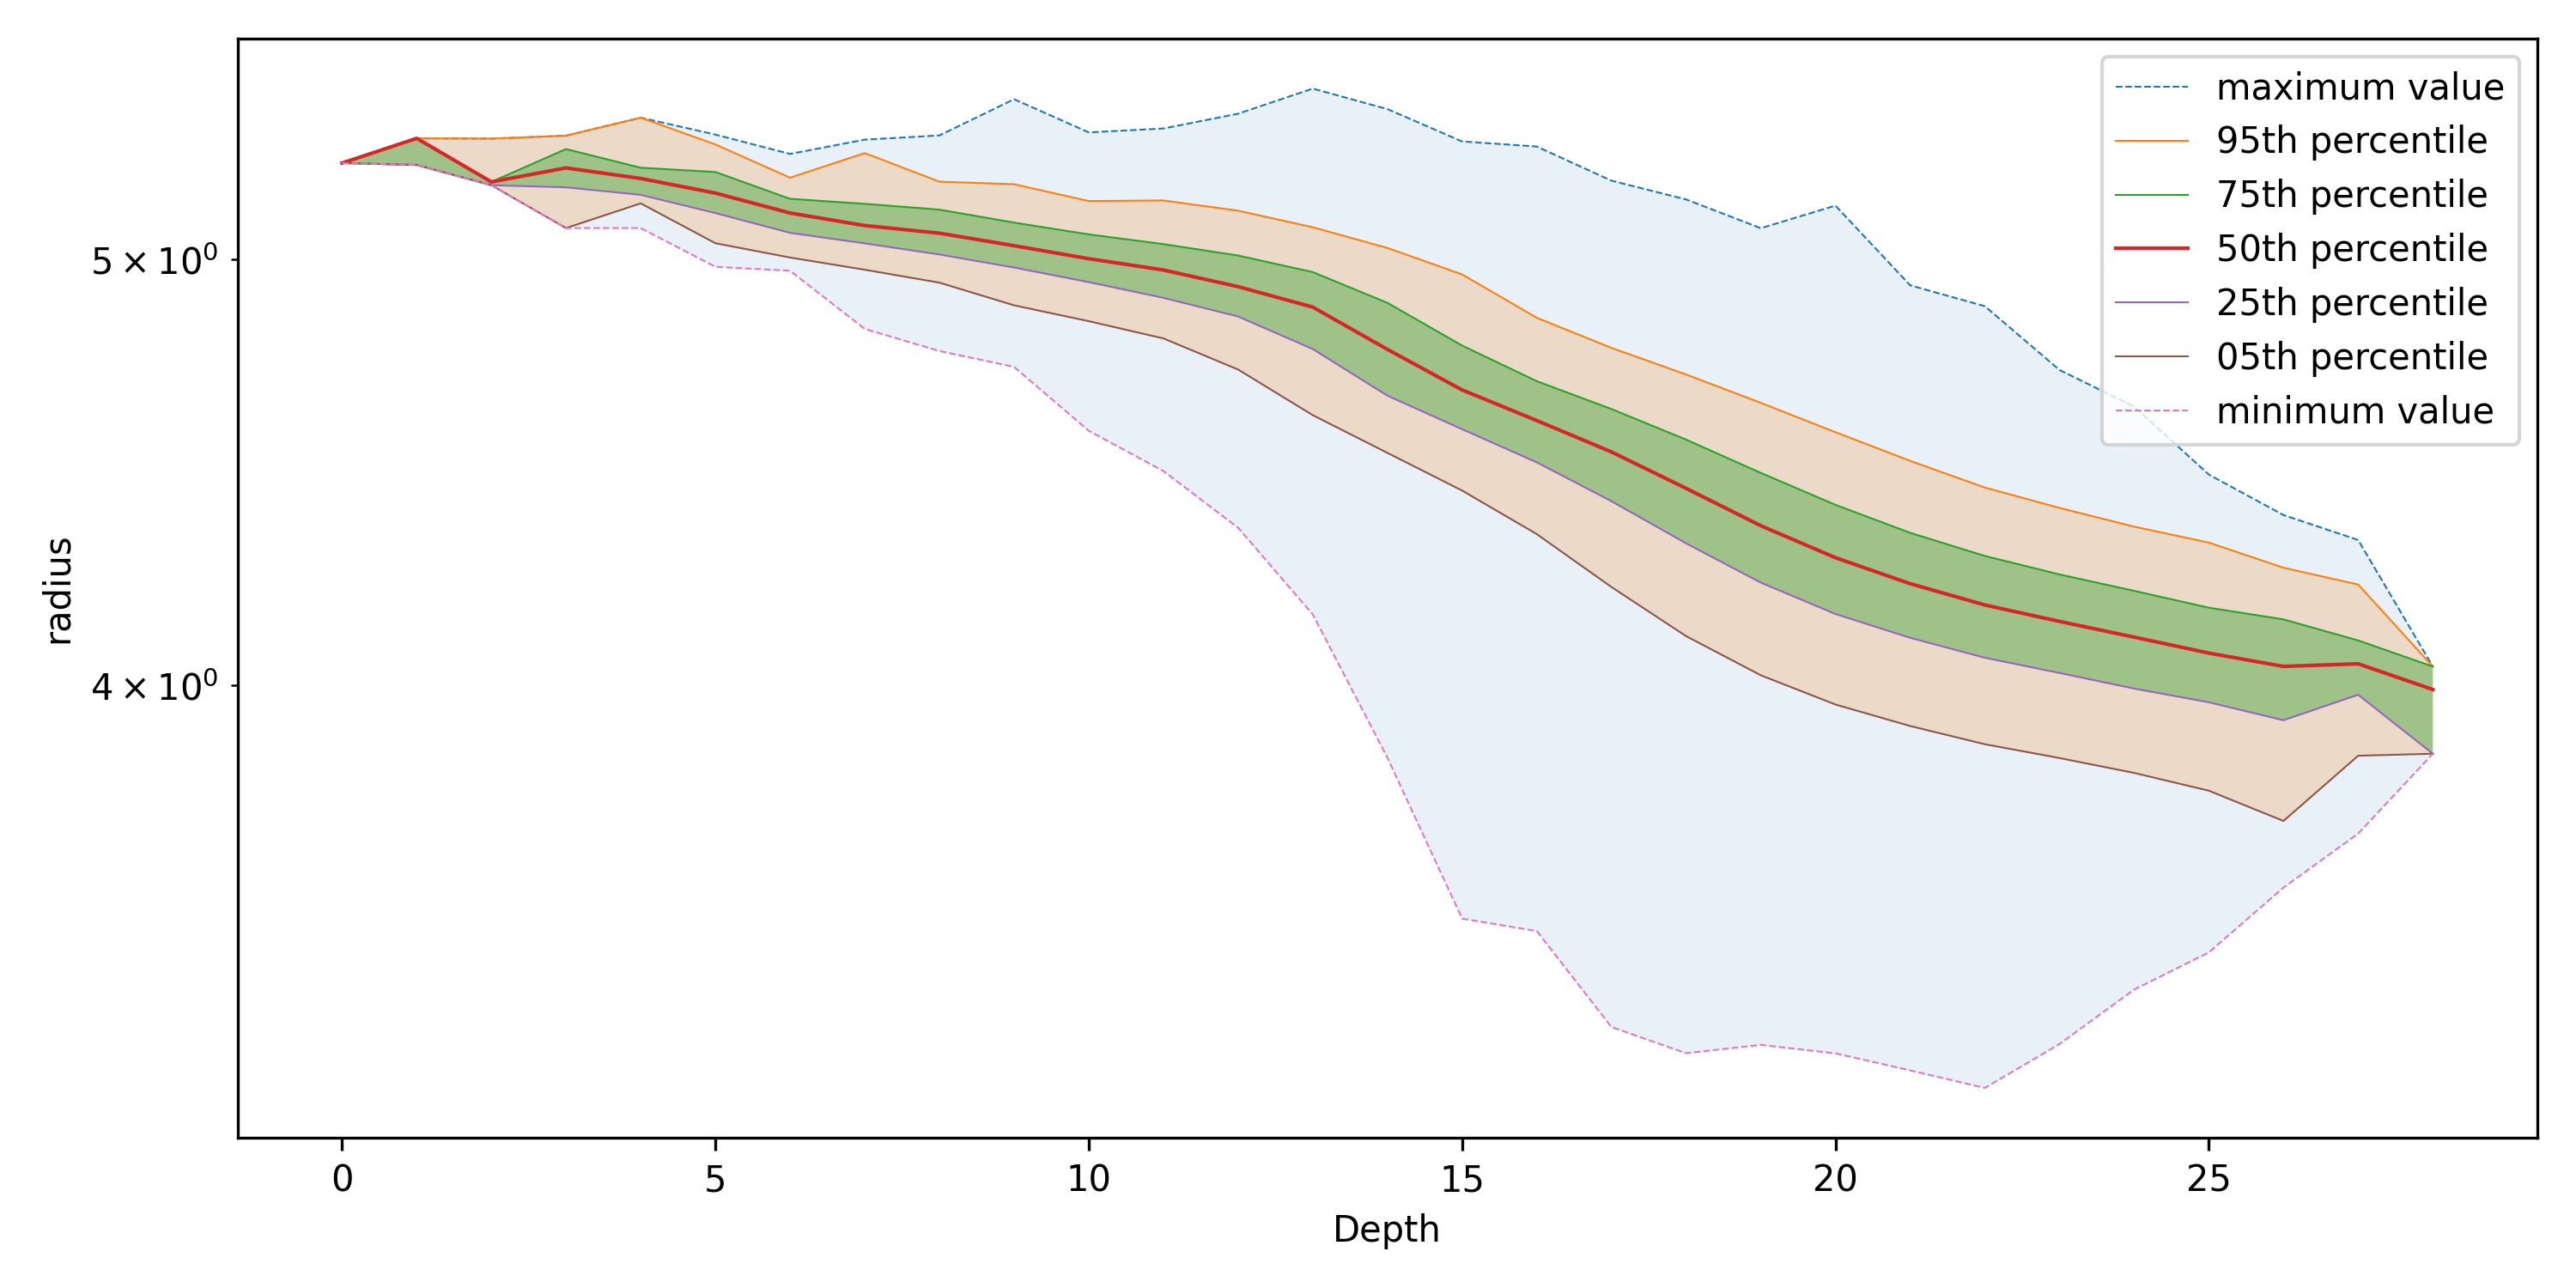
\includegraphics[width=0.95\textwidth]{images/radius/random-1000000.png}\\
    \subcaption{A random dataset}
    \label{fig:results:random-radius}
    \end{subfigure}
    \vspace{1em}
    \caption{Radius vs. cluster depth across six datasets, grouped by decile of radius and weighted by the cardinalities of the clusters.
    The last dataset is randomly generated.}
    \label{fig:results:radius-plots}
\end{figure}

\begin{figure}[ht!]
    \begin{subfigure}[b]{0.47\textwidth}
    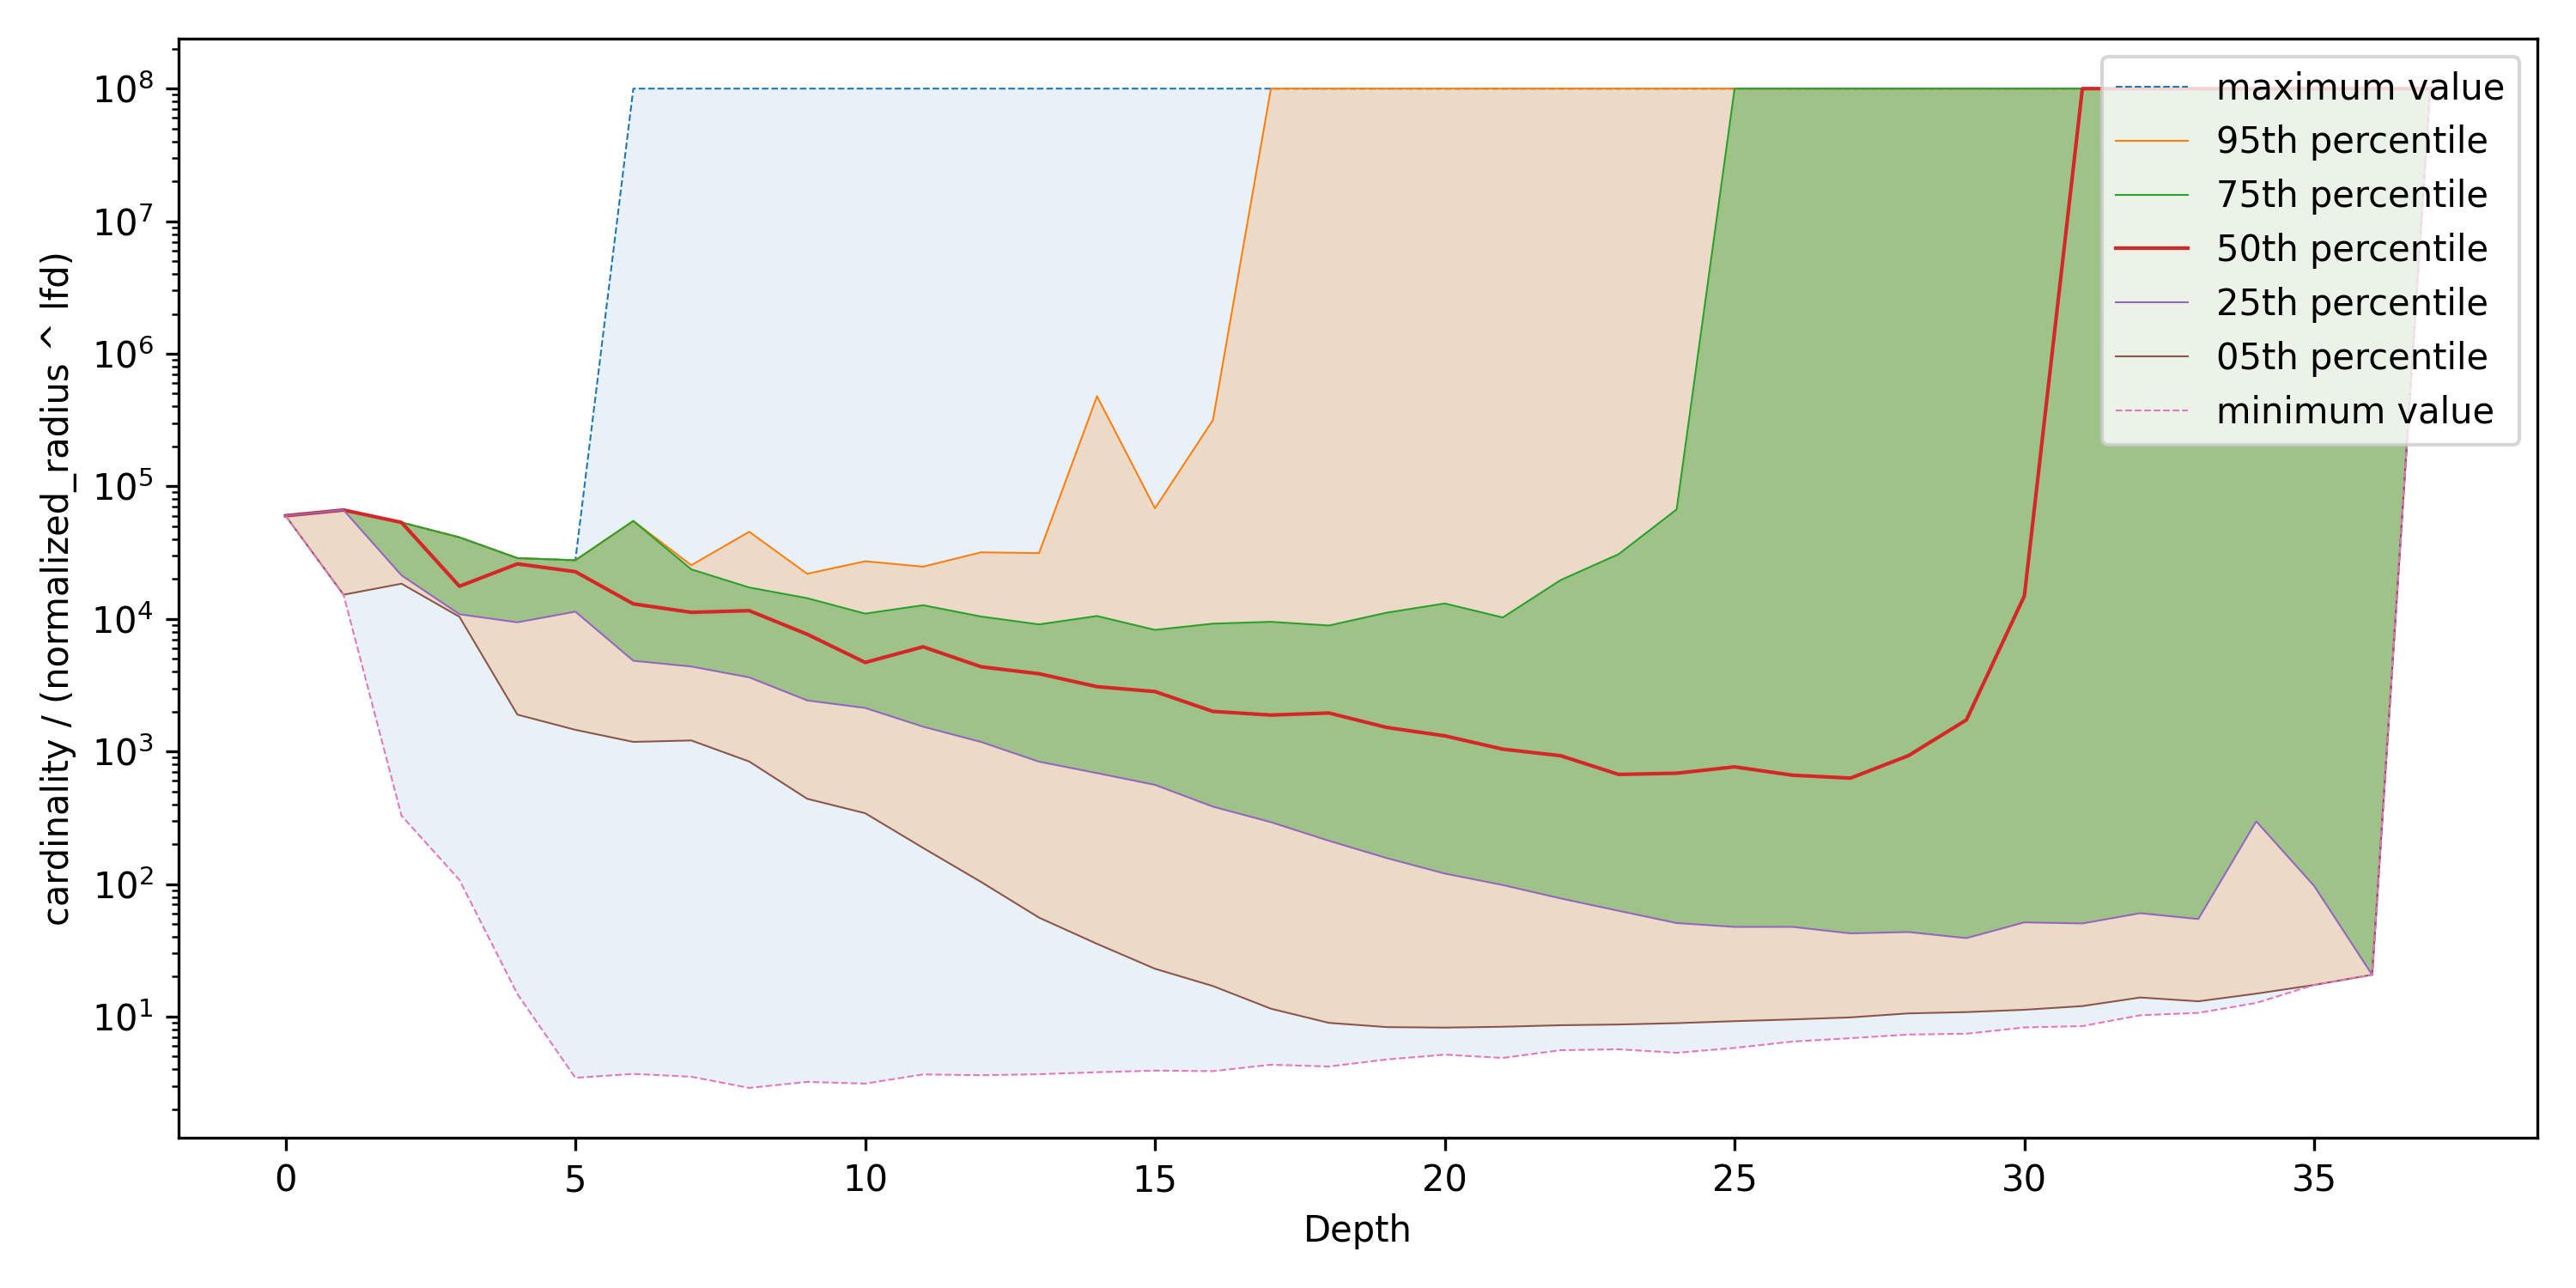
\includegraphics[width=0.95\textwidth]{images/fractal_density/fashion-mnist-60000.png}\\
    \subcaption{Fashion-mnist}
    \label{fig:results:fashion-mnist-fractal_density}
    \end{subfigure}%
    \begin{subfigure}[b]{0.47\textwidth}
    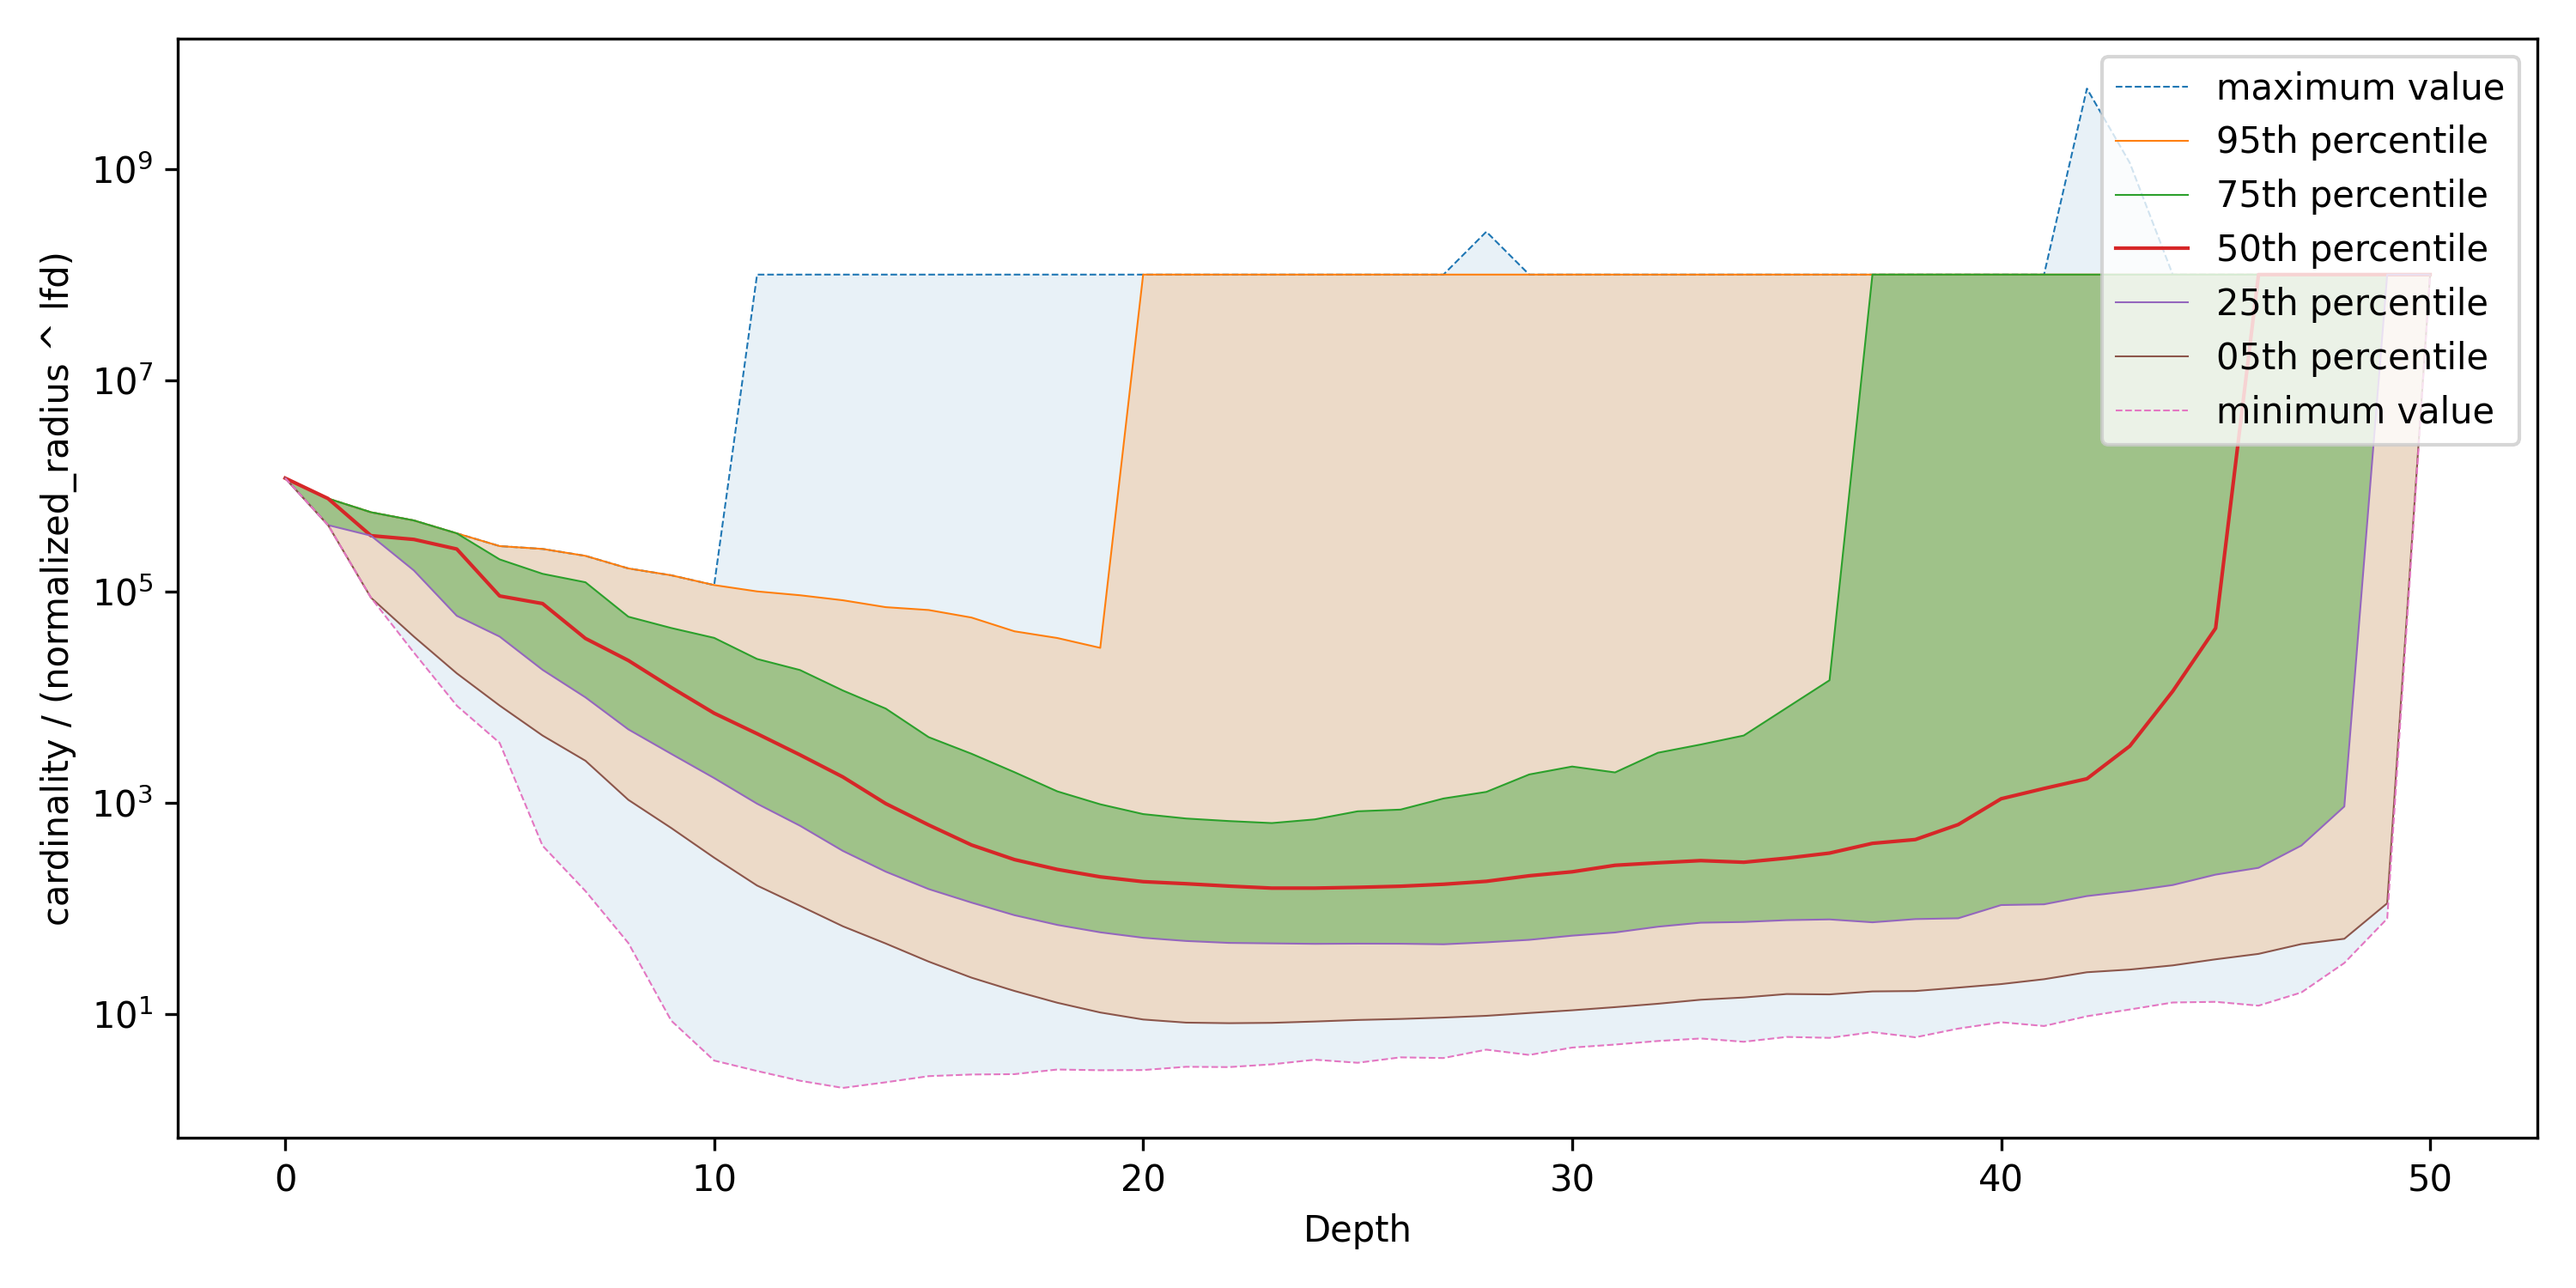
\includegraphics[width=0.95\textwidth]{images/fractal_density/glove-25-1183514.png}\\
    \subcaption{Glove-25}
    \label{fig:results:glove-25-fractal_density}
    \end{subfigure}
    \vspace{1em}
    \\
    \begin{subfigure}[b]{0.47\textwidth}
    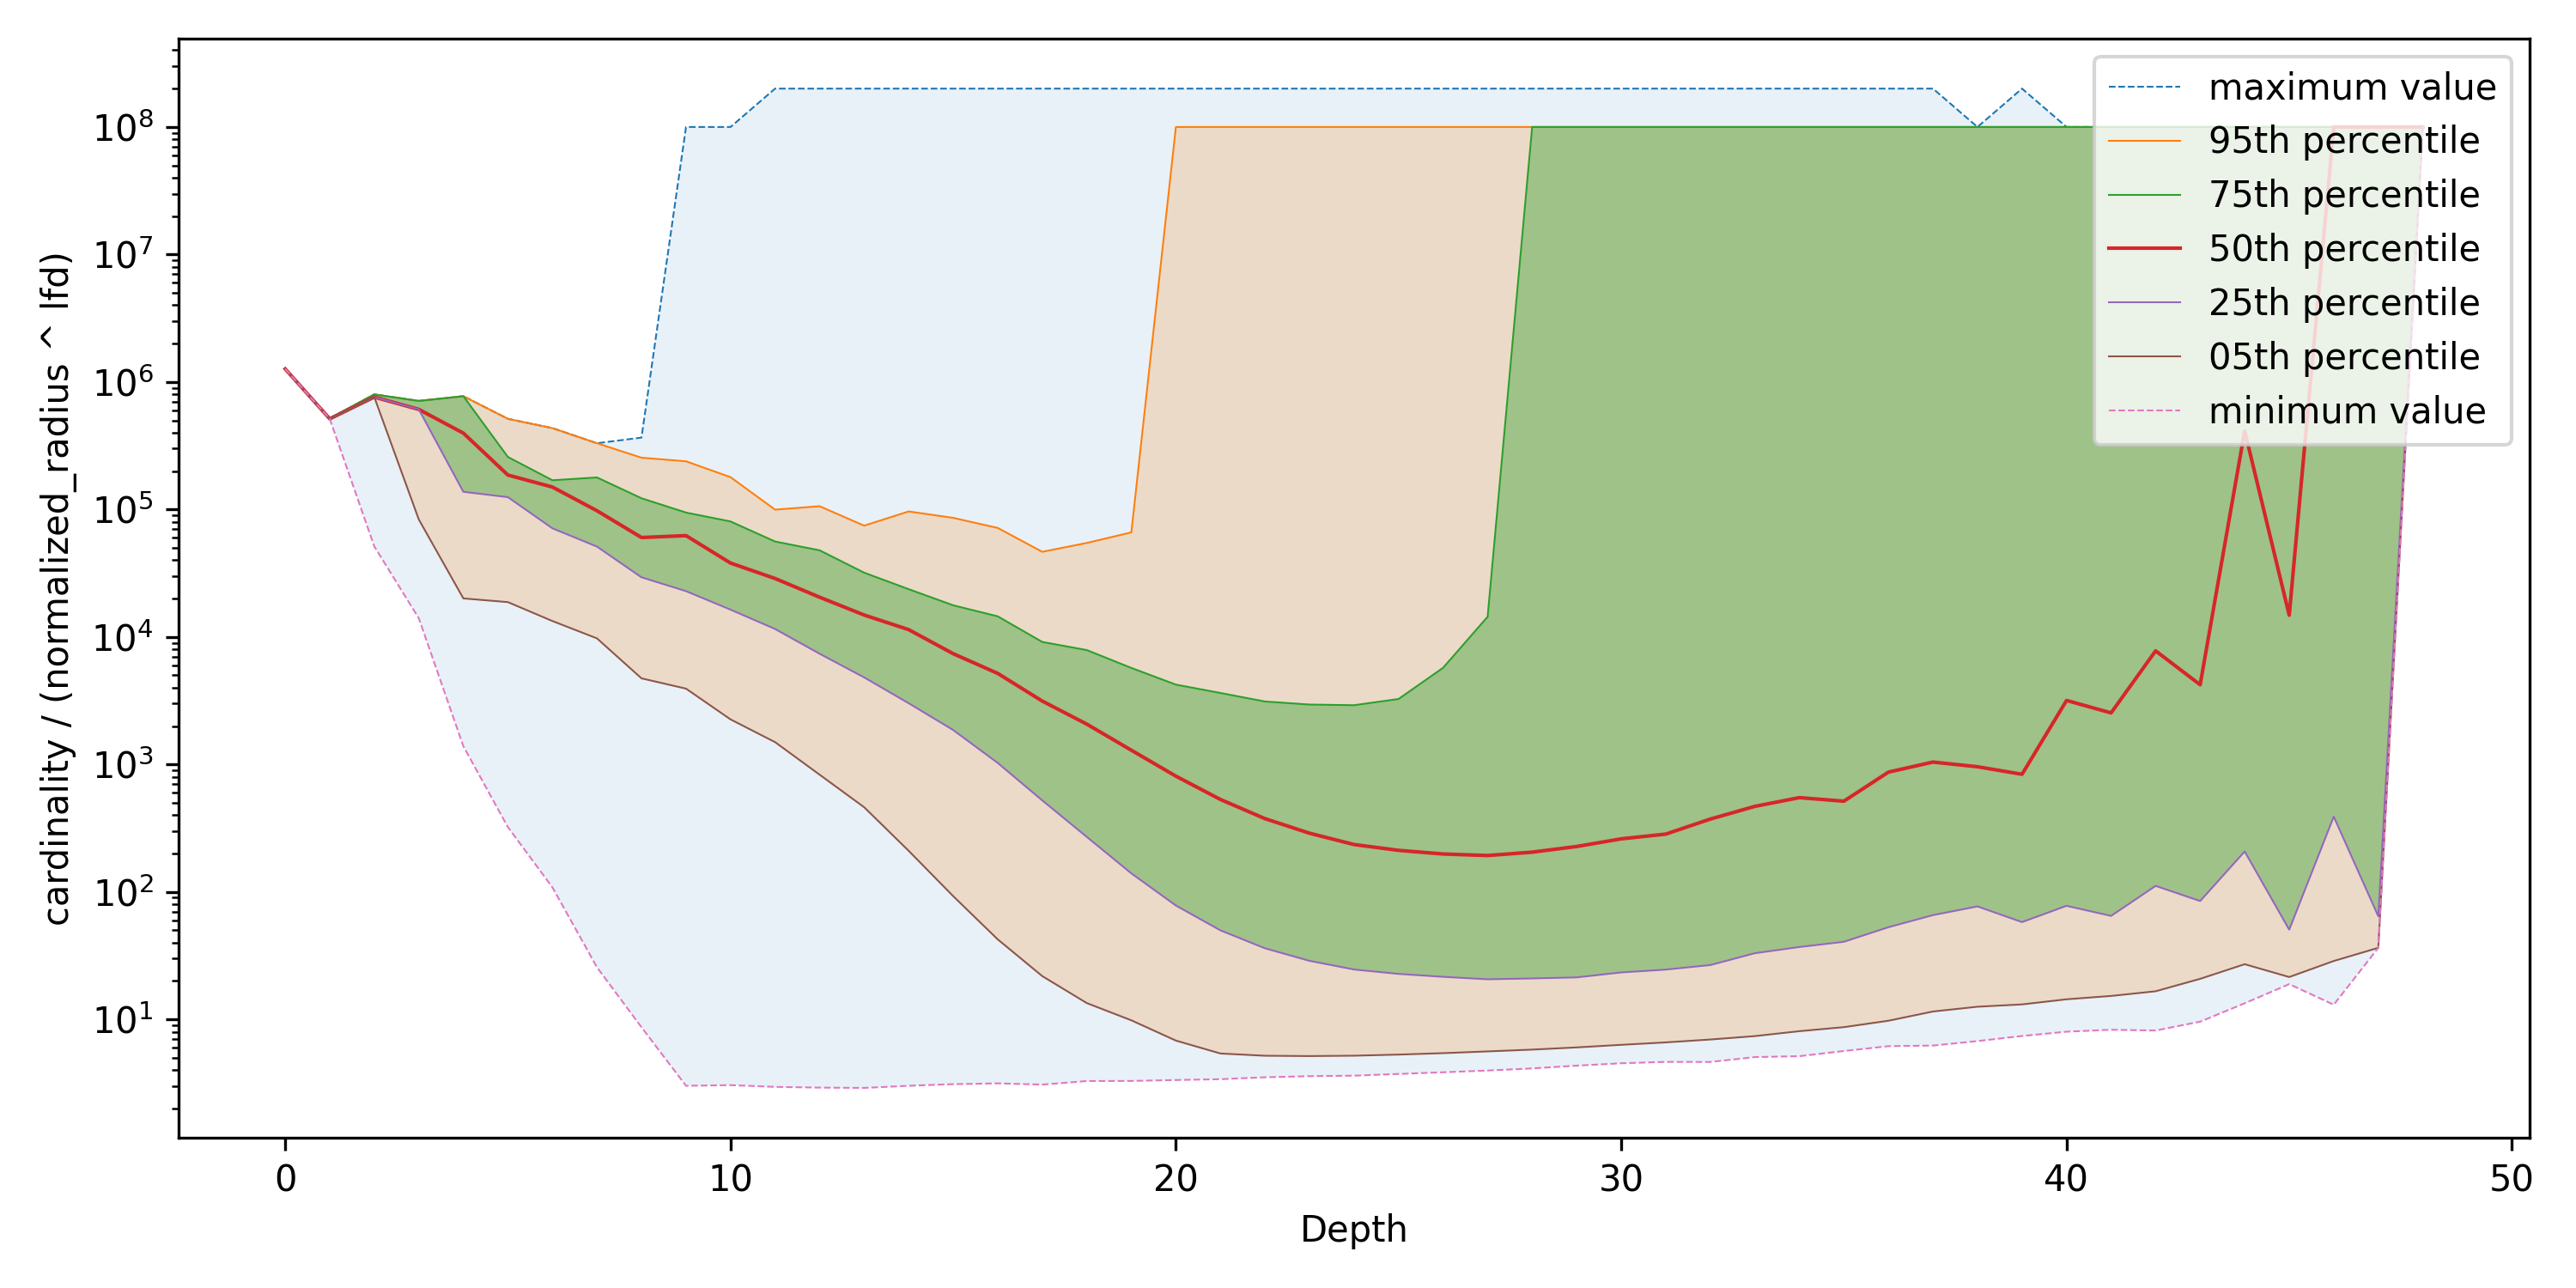
\includegraphics[width=0.95\textwidth]{images/fractal_density/sift-1000000.png}\\
    \subcaption{Sift}
    \label{fig:results:sift-fractal_density}
    \end{subfigure}%
    \begin{subfigure}[b]{0.47\textwidth}
    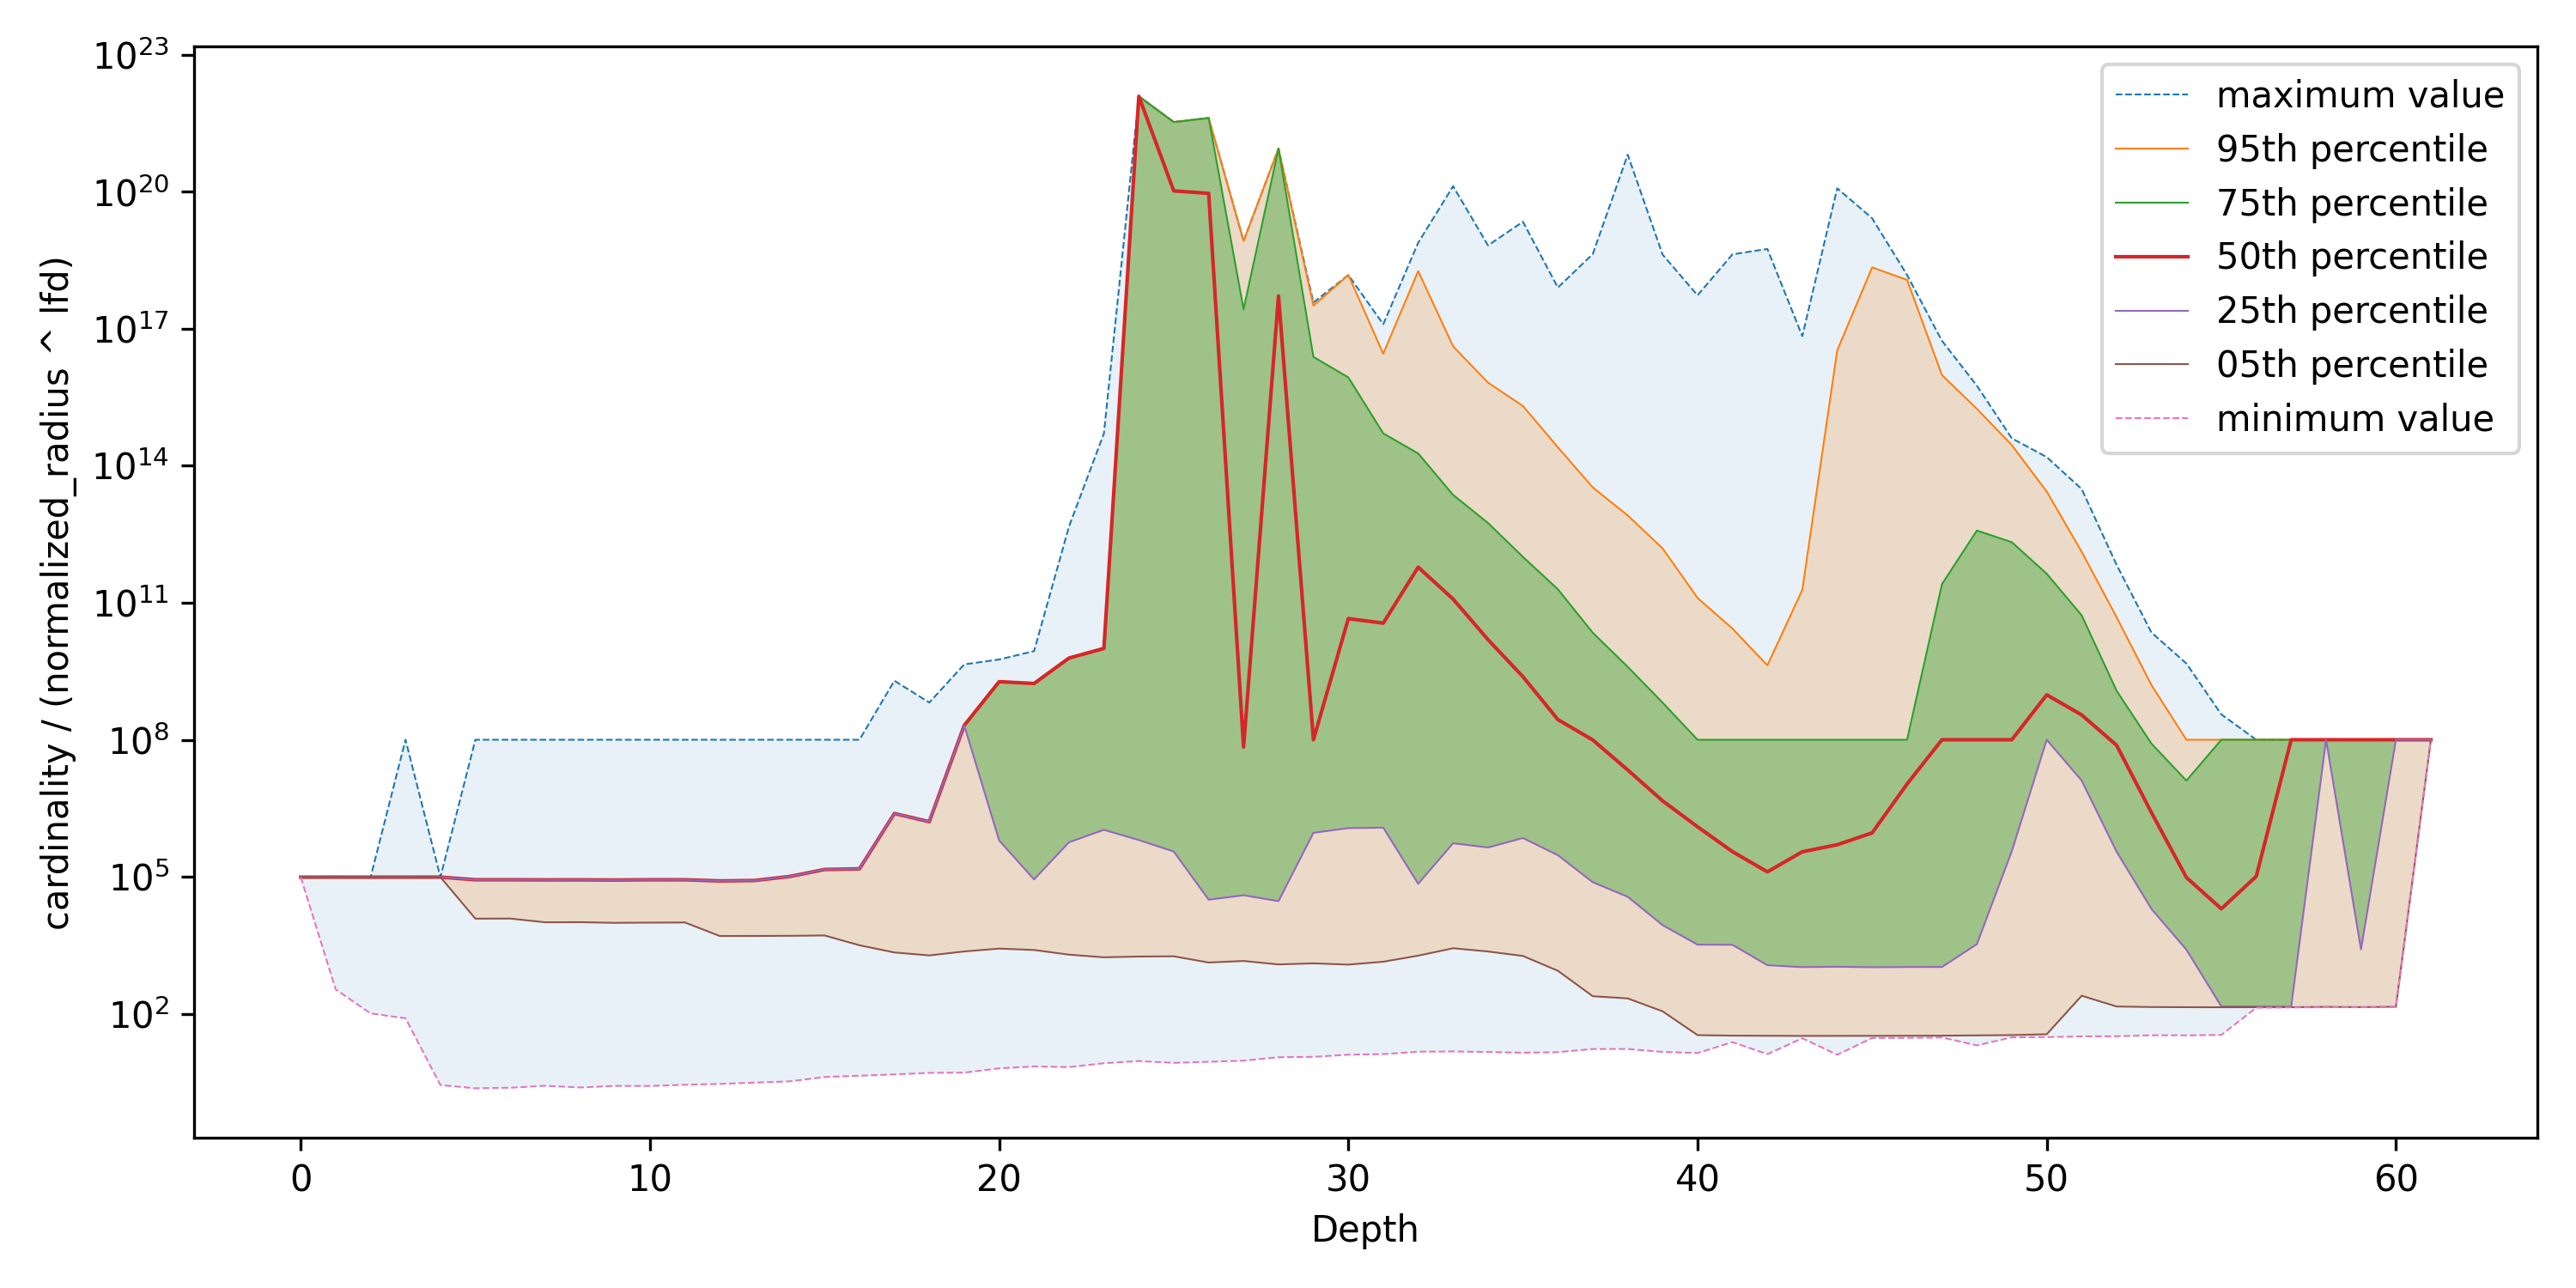
\includegraphics[width=0.95\textwidth]{images/fractal_density/radio-ml-97920.png}\\
    \subcaption{RadioML}
    \label{fig:results:radioml-fractal_density}
    \end{subfigure}%
    \\
    \begin{subfigure}[b]{0.47\textwidth}
    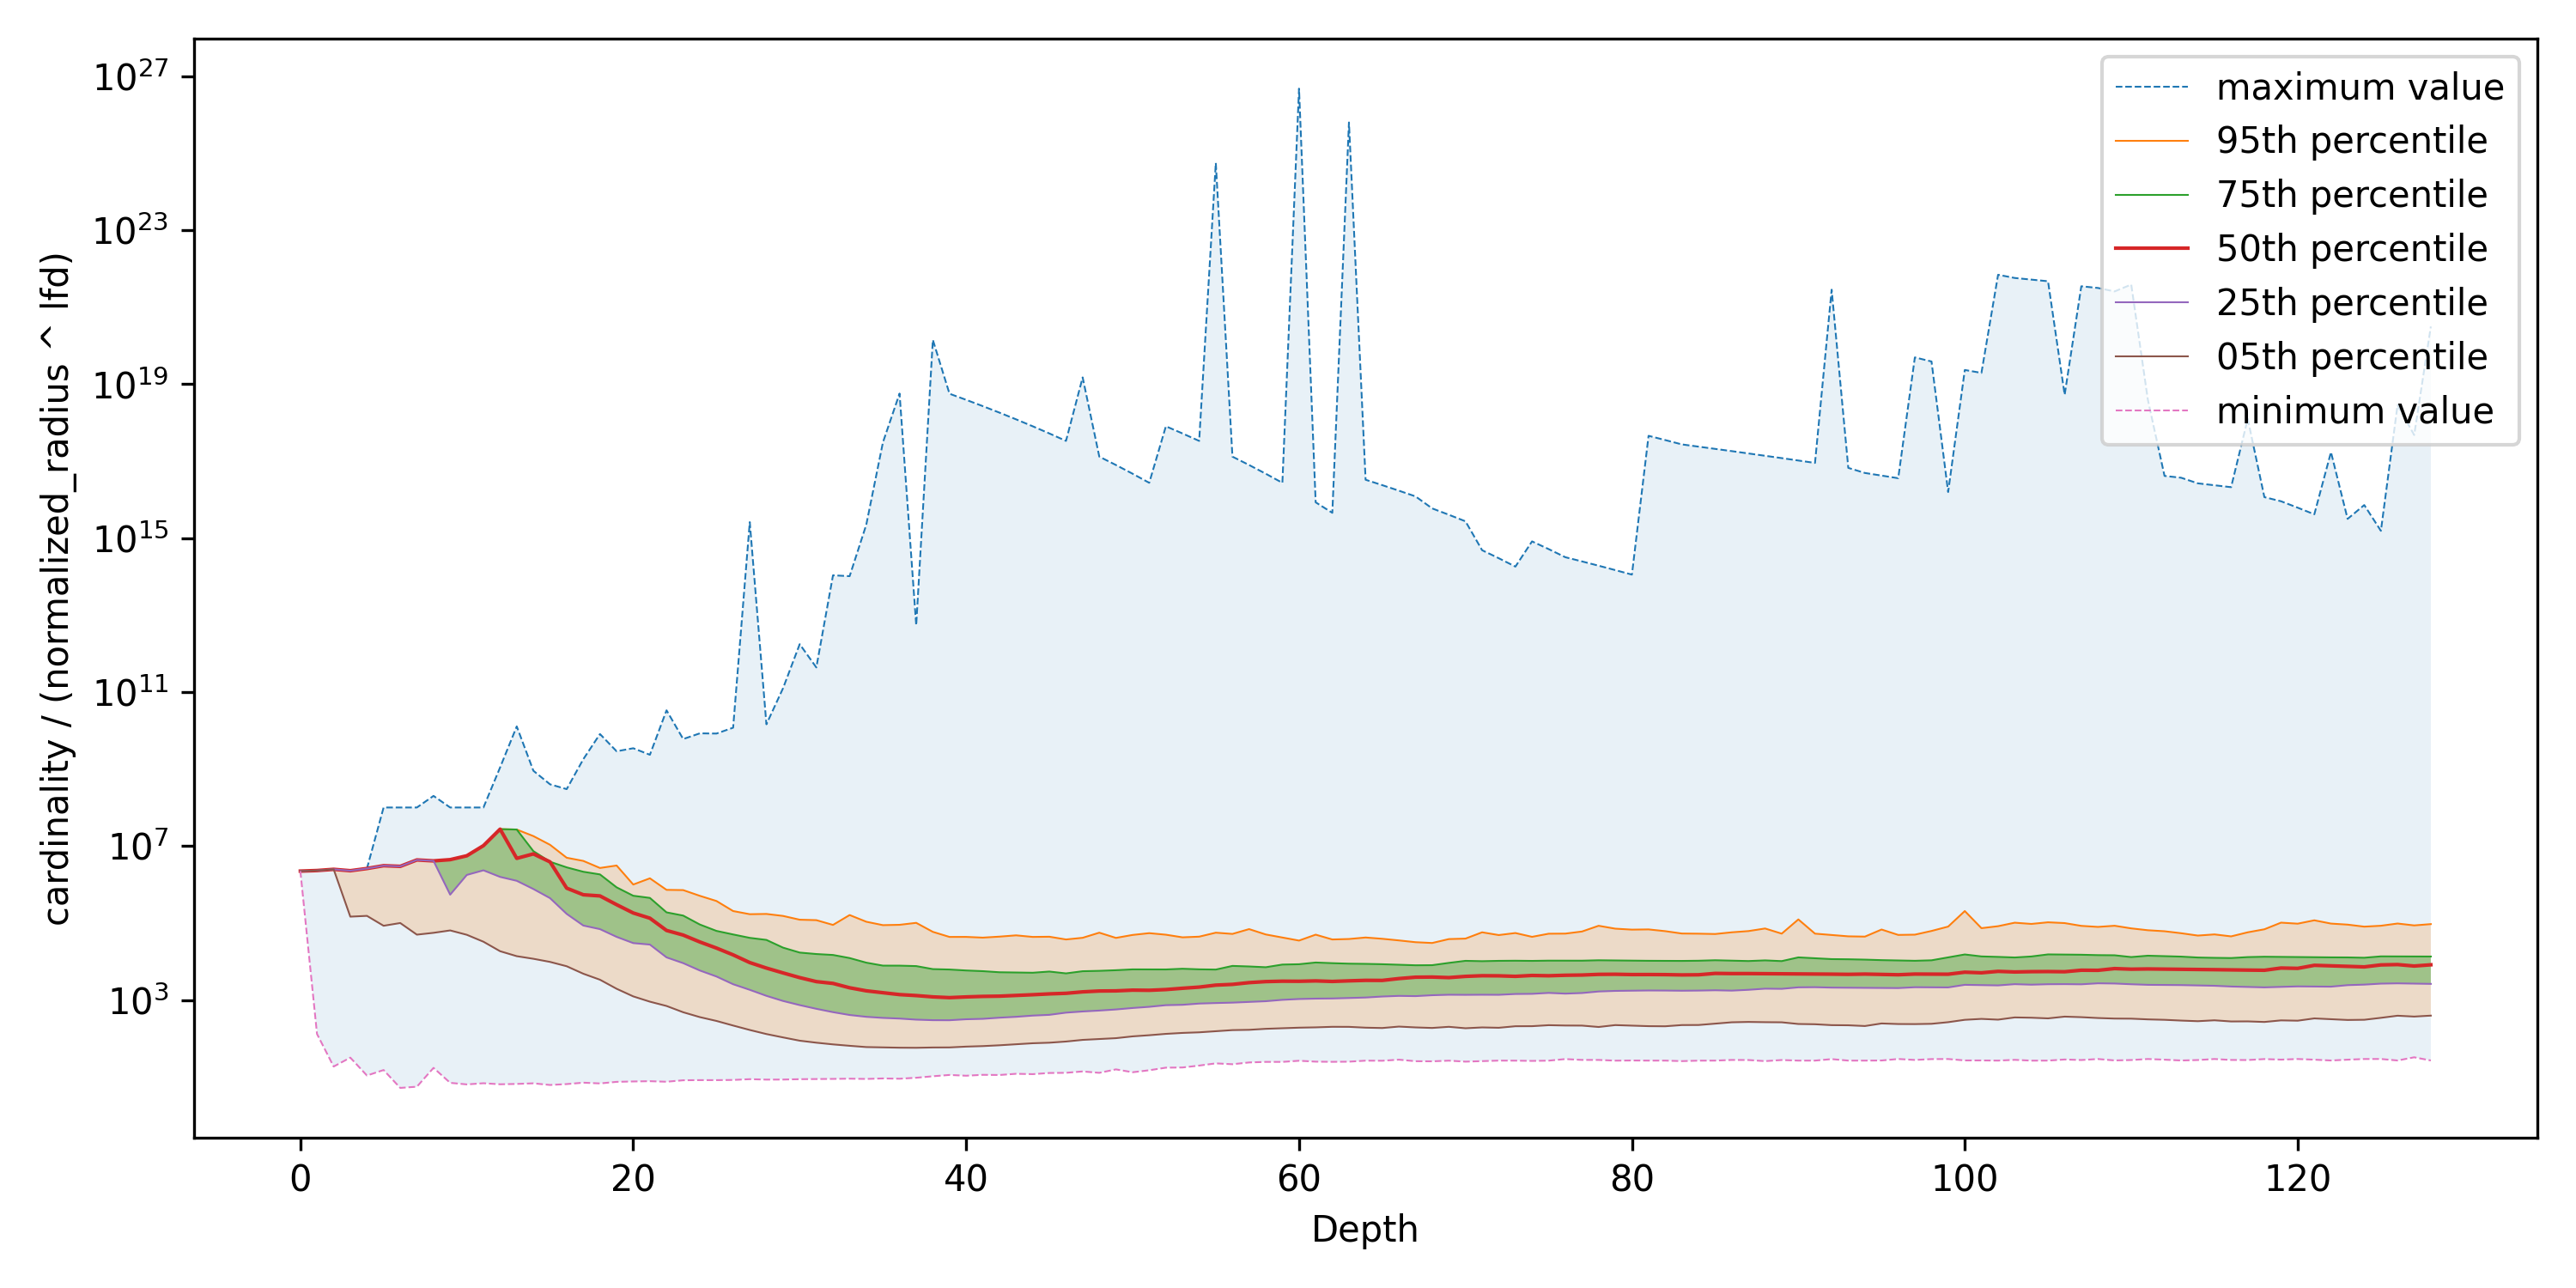
\includegraphics[width=0.95\textwidth]{images/fractal_density/silva-2224640.png}\\
    \subcaption{Silva 18S}
    \label{fig:results:silva-fractal_density}
    \end{subfigure}%
    \begin{subfigure}[b]{0.47\textwidth}
    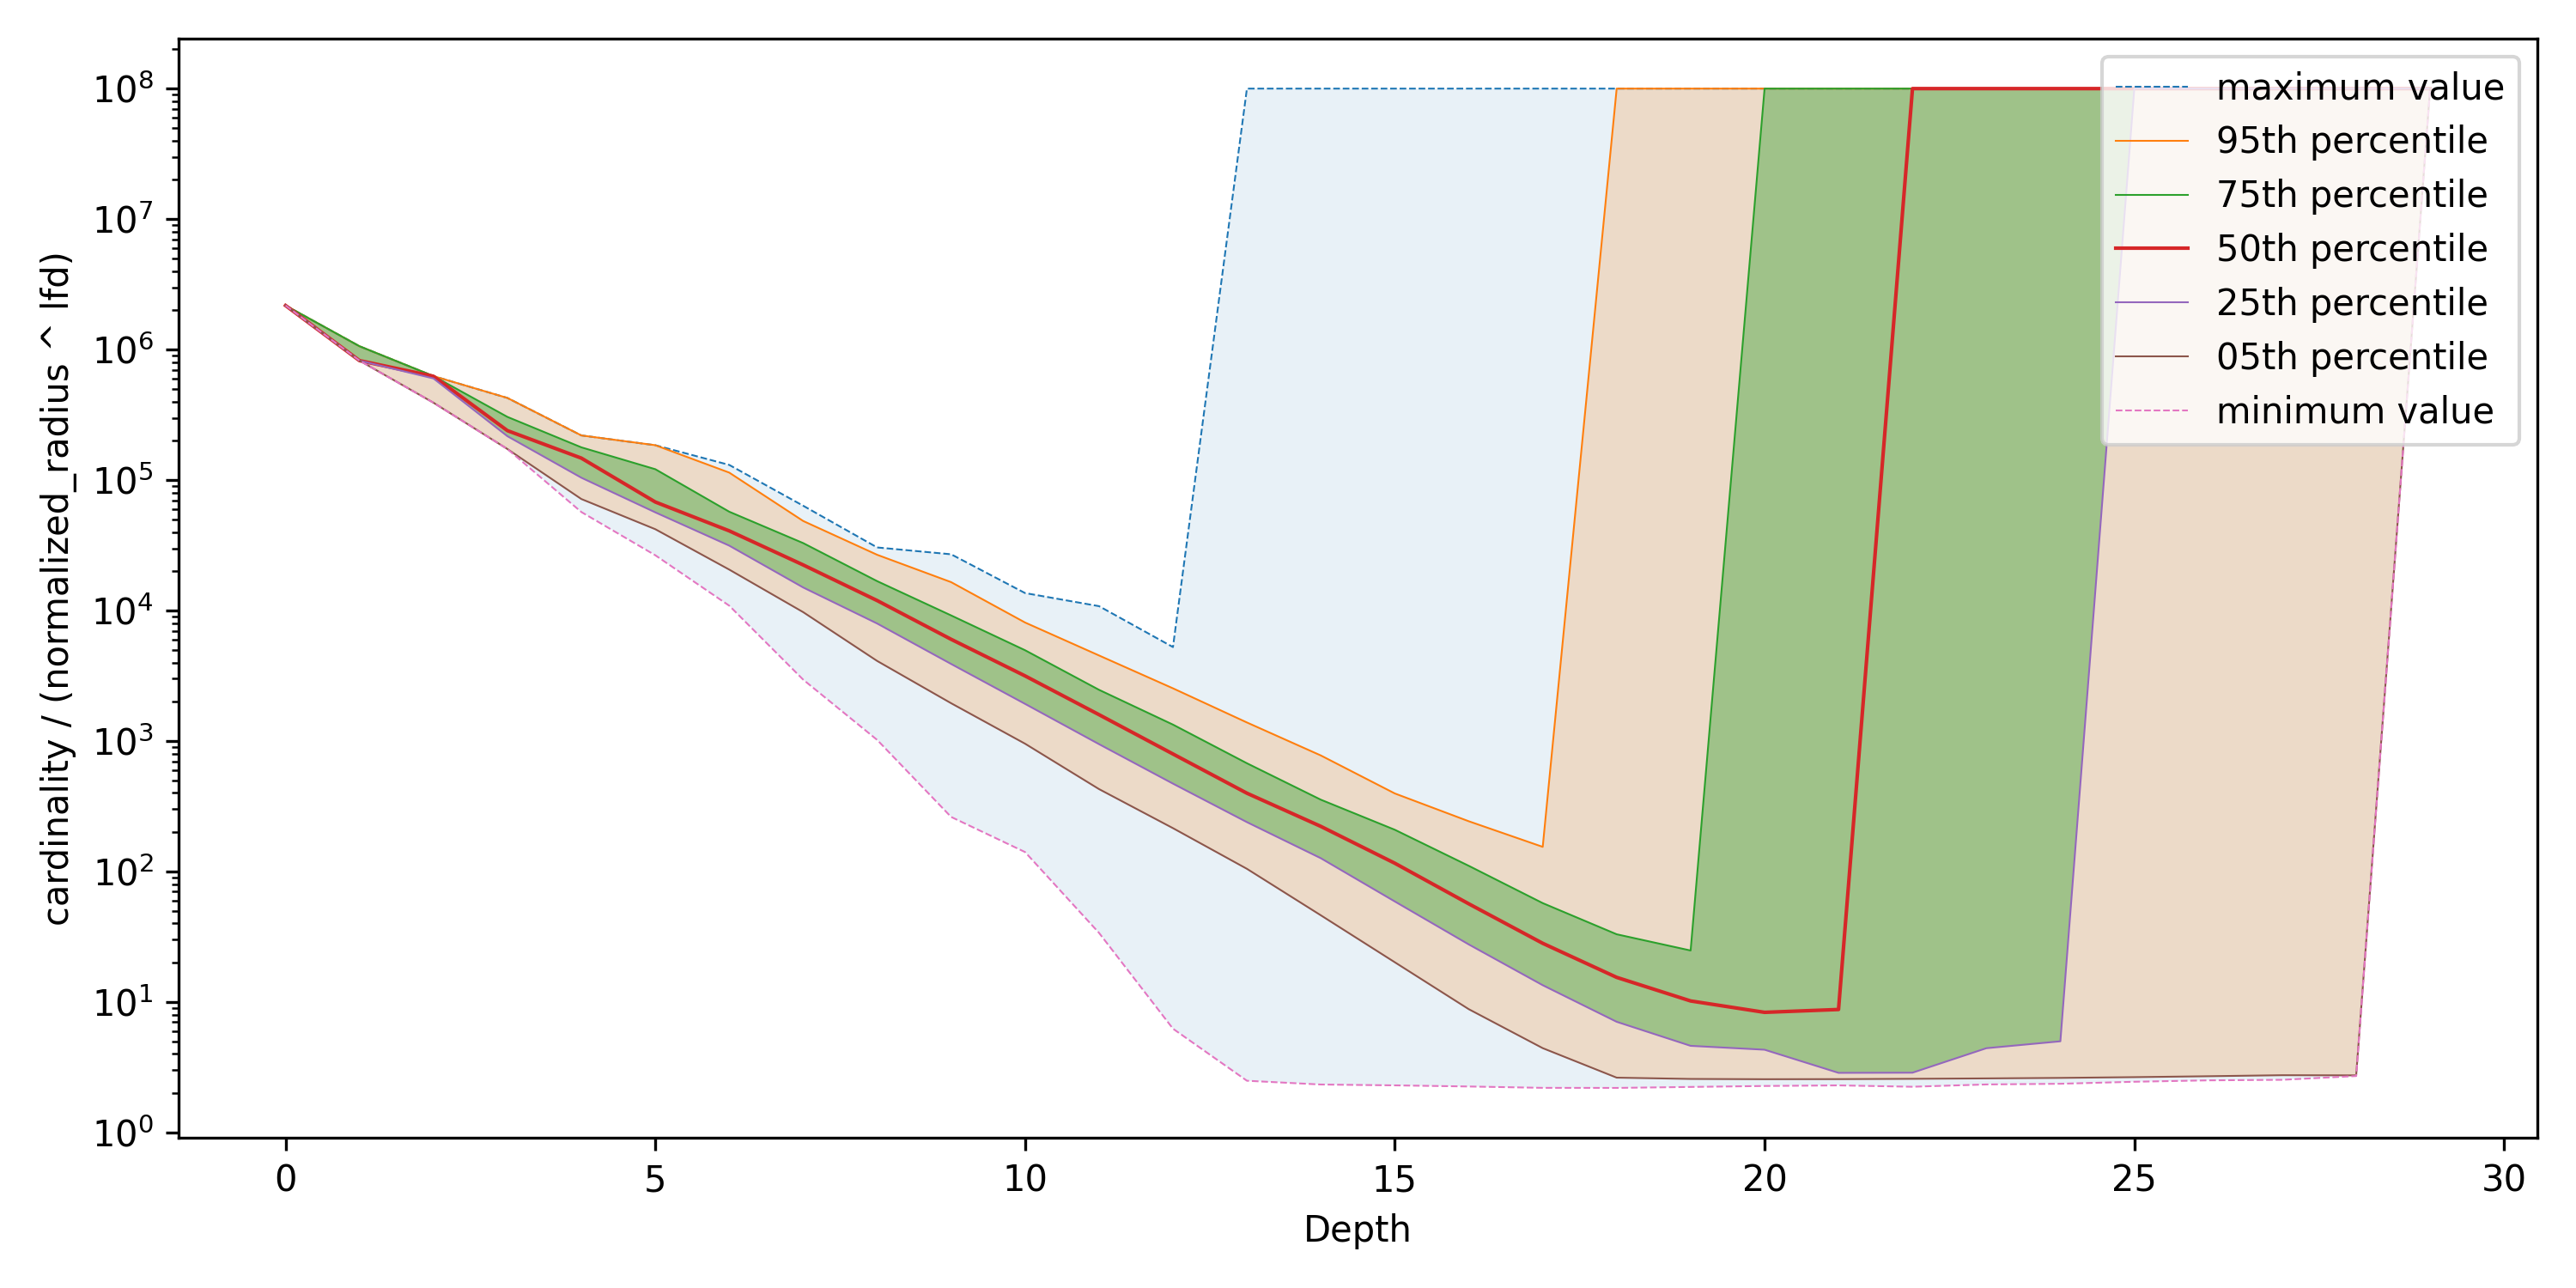
\includegraphics[width=0.95\textwidth]{images/fractal_density/random-1000000.png}\\
    \subcaption{A random dataset}
    \label{fig:results:random-fractal_density}
    \end{subfigure}
    \vspace{1em}
    \caption{Fractal Density vs. cluster depth across six datasets, grouped by decile of fractal density and weighted by the cardinalities of the clusters.
    The last dataset is randomly generated.
    Fractal Density is defined as $\frac{cardinality}{radius^{LFD}}$}
    \label{fig:results:fractal_density-plots}
\end{figure}


\bibliographystyle{siamplain}
\bibliography{references}


\end{document}
